
% \includeonly non esclude i capitoli 4-6, li salta soltanto in composizione:
% LaTeX ne legge comunque i file .aux, quindi i rimandi in avanti ("sezione
% 4.2", "sezione 5.1", ...) continuano a mostrare il numero giusto e l'indice
% resta quello completo.
%
% VINCOLO: questo file va compilato DOPO almeno una compilazione di
% Tesi_Corsi_Leonardo_656276.tex, che e' quella che produce gli .aux dei
% capitoli 4-6. Su una cartella pulita i rimandi in avanti darebbero "??".
%
%   latexmk -pdf Tesi_Corsi_Leonardo_656276.tex
%   latexmk -pdf Tesi_capitoli_1-3.tex

% !TEX root = Tesi_Corsi_Leonardo_656276.tex
% Preambolo condiviso fra la tesi completa e il PDF dei soli capitoli 1-3.
% Non contiene \begin{document}: lo apre corpo.tex.

% Template Tesi in Informatica, ispirata al template "Tesi di laurea - Università di Pisa" di Simone Schirinzi (https://www.overleaf.com/latex/templates/tesi-di-laurea-universita-di-pisa/rwdcqtqwftpg).

% Carattere dimensione 12
\documentclass[12pt]{report}

% Per la stampa fronte-retro sostituire con:
% \documentclass[12pt, twoside]{report}

% Margini (4cm a sx, 2.5cm a dx, 2.5cm in alto, 2.5cm in basso)
% head=21.75pt: spazio per la testatina, il valore richiesto da scrlayer-scrpage
\usepackage[top=2.5cm, bottom=2.5cm, left=4cm, right=2.5cm, head=21.75pt, centering]{geometry}

% Per la stampa fronte-retro sostituire con: 
% \usepackage[top=2.5cm, bottom=2.5cm, inner=4cm, outer=4cm, right=2.5cm, centering]{geometry}

% Interlinea
\linespread{1.5}

% Librerie utili
\usepackage[italian]{babel} % applicazione regole di scrittura per la lingua italiana 
\usepackage[utf8]{inputenc} % codifica UTF-8
\usepackage{scrlayer-scrpage} % stili pagina: testatine e pie' di pagina
% Testatina: capitolo a sinistra, numero di pagina a destra, riga di separazione.
% Le pagine di apertura capitolo restano senza testatina (stile plain) e il
% numero di pagina lo tengono in fondo: e' la forma fra parentesi quadre.
\automark[section]{chapter}
\ihead[]{\headmark}
\chead[]{}
\ohead[]{\pagemark}
\ifoot[]{}
\cfoot[]{}
\ofoot[\pagemark]{}
\KOMAoptions{headsepline=true}
\pagestyle{scrheadings}
\usepackage{mathptmx} % font Times New Roman (simile)
\usepackage{graphicx} % inserimento di immagini
\usepackage{csquotes} % per le citazioni "in blocco"
\usepackage{url} % per \url{} nelle voci di bibliografia
%\usepackage[backend=biber, sorting=nty, ]{biblatex} % bibliografia con pacchetto biblatex (https://ctan.org/pkg/biblatex?lang=en)
\appto{\bibsetup}{\raggedright}

\usepackage{titlesec} % per la formattazione dei titoli delle sezioni, capitoli etc.
\usepackage{float} % per il posizionamento delle immagini
\usepackage{booktabs} % \toprule \midrule \bottomrule per le tabelle dei risultati
\usepackage{enumitem} % spaziatura degli elenchi: \begin{itemize}[topsep=..., itemsep=...]
\usepackage{needspace} % \needspace{N\baselineskip}: non spezzare un blocco a fine pagina
\usepackage{tikz} % per i disegni dell'architettura
\usetikzlibrary{arrows.meta, calc}
\usepackage{pgfplots} % per i grafici delle misure
\pgfplotsset{compat=1.18}
\usepackage{amsmath} % per le formule dei costi
\usepackage{amssymb} % \square a fine dimostrazione

\usepackage{listings} % per il codice di programmazione
% Fonte https://en.wikibooks.org/wiki/LaTeX/Source_Code_Listings. Per la lista di sintassi riconosciute.
\renewcommand{\lstlistingname}{Codice}% Listing -> Codice
\usepackage{xcolor}  % stile del codice
\definecolor{mygreen}{rgb}{0,0.6,0}
\definecolor{mygray}{rgb}{0.5,0.5,0.5}
\definecolor{mymauve}{rgb}{0.58,0,0.82}
\definecolor{darkgray}{rgb}{.4,.4,.4}
\definecolor{navy}{HTML}{000080}
\definecolor{purple}{rgb}{0.65, 0.12, 0.82}
\definecolor{codepurple}{rgb}{0.58,0,0.82}
\definecolor{backcolour}{rgb}{0.95,0.95,0.92}

% Stili configurabili del codice (lslisting) 
\lstset{ %
belowcaptionskip=0.5em,
backgroundcolor=\color{backcolour}, % choose the background color; you must add \usepackage{color} or \usepackage{xcolor}
basicstyle=\footnotesize, % the size of the fonts that are used for the code
breakatwhitespace=false, % sets if automatic breaks should only happen at whitespace
breaklines=true, % sets automatic line breaking
captionpos=b, % sets the caption-position to bottom
commentstyle=\color{mygreen}, % comment style
deletekeywords={...}, % if you want to delete keywords from the given language
escapeinside={\%*}{*)}, % if you want to add LaTeX within your code
extendedchars=true, % lets you use non-ASCII characters; for 8-bits encodings only, does not work with UTF-8
frame=single, % adds a frame around the code
keepspaces=true, % keeps spaces in text, useful for keeping indentation of code (possibly needs columns=flexible)
keywordstyle=\color{codepurple}, % keyword style
% language=Octave, % the language of the code
morekeywords={*,...}, % if you want to add more keywords to the set
numbers=left, % where to put the line-numbers; possible values are (none, left, right)
numbersep=5pt, % how far the line-numbers are from the code
numberstyle=\tiny\color{mygray}, % the style that is used for the line-numbers
rulecolor=\color{black}, % if not set, the frame-color may be changed on line-breaks within not-black text (e.g. comments (green here))
showspaces=false, % show spaces everywhere adding particular underscores; it overrides 'showstringspaces'
showstringspaces=false, % underline spaces within strings only
showtabs=false, % show tabs within strings adding particular underscores
stepnumber=1, % the step between two line-numbers. If it's 1, each line will be numbered
stringstyle=\color{mymauve}, % string literal style
tabsize=2, % sets default tabsize to 2 spaces
title=\lstname % show the filename of files included with \lstinputlisting; also try caption instead of title
}

% END of listing package 

% Esempio riconoscimento sintassi JavaScript 

\lstdefinelanguage{JavaScript}{
  keywords={typeof, new, true, false, catch, function, return, null, catch, switch, var, const, let, if, in, while, do, else, case, break},
  keywordstyle=\color{blue}\bfseries,
  ndkeywords={class, export, boolean, throw, implements, import, this},
  ndkeywordstyle=\color{darkgray}\bfseries,
  identifierstyle=\color{black},
  sensitive=false,
  comment=[l]{//},
  morecomment=[s]{/*}{*/},
  commentstyle=\color{mygreen}\ttfamily,
  stringstyle=\color{red}\ttfamily,
  morestring=[b]',
  morestring=[b]"
}

% Assembly RISC-V: le istruzioni rv32i usate dai kernel, piu' le quattro
% istruzioni di comunicazione dell'estensione, evidenziate a parte.
\lstdefinelanguage{RISCV}{
  keywords={add, addi, sub, and, andi, or, ori, xor, xori, sll, slli, srl, srli,
            sra, srai, slt, slti, sltu, sltiu, lui, auipc, lw, lh, lhu, lb, lbu,
            sw, sh, sb, beq, bne, blt, bge, bltu, bgeu, beqz, bnez, blez, bgez,
            j, jal, jalr, mv, li, la, ret, nop, ecall, mul},
  keywordstyle=\color{codepurple}\bfseries,
  ndkeywords={IN, OUT, ISRDY, SETRDY, NORD, EST, SUD, OVEST},
  ndkeywordstyle=\color{navy}\bfseries,
  identifierstyle=\color{black},
  sensitive=true,
  comment=[l]{\#},
  commentstyle=\color{mygreen}\ttfamily,
  morestring=[b]",
  stringstyle=\color{mymauve}\ttfamily
}

\lstset{
   extendedchars=true,
   basicstyle=\footnotesize\ttfamily,
   showstringspaces=false,
   showspaces=false,
   numbers=left,
   numberstyle=\footnotesize,
   numbersep=9pt,
   tabsize=2,
   breaklines=true,
   showtabs=false,
   captionpos=b
   % I listati sono oggetti mobili, cosi' non vengono mai spezzati fra due
   % pagine e la didascalia resta attaccata al codice. La chiave 'float' NON
   % ha effetto se data qui: va messa nell'argomento opzionale di ogni
   % lstlisting, e li' infatti c'e'. Un 'float=htbp' in questo blocco lascia
   % credere di coprire il caso senza coprirlo, quindi non c'e'.
}

% Nessuna riga vedova o orfana: una riga sola staccata dal suo paragrafo
% e' il difetto di impaginazione piu' visibile in un testo interlinea 1,5
\widowpenalty=10000
\clubpenalty=10000

% Nessun oggetto mobile scavalca l'inizio di una sottosezione. Senza questa
% barriera un listato o una figura che non entrano nella pagina corrente
% vengono rinviati alla prima posizione utile, che puo' cadere DOPO il titolo
% della sottosezione seguente: il codice di reduce finiva sotto il titolo di
% matmul, dove si legge come se fosse di matmul. L'opzione [section] copre i
% titoli di sezione, la ridefinizione sotto quelli di sottosezione.
\usepackage[section]{placeins}
\let\originalsubsection\subsection
\renewcommand{\subsection}{\FloatBarrier\originalsubsection}

% Didascalie: etichetta (Figura 3.1, Codice 3.2, Tabella 5.4) in grassetto e
% testo in corsivo, cosi' le didascalie lunghe si staccano dal corpo del testo.
% Caricato dopo 'listings' perche' valga anche per i lstlisting.
\usepackage{caption}
\captionsetup{labelfont=bf, textfont=it}

% Parametri dei float. Con i valori predefiniti una figura alta piu' di meta'
% pagina finisce su una pagina tutta sua, con fasce bianche sopra e sotto:
% questi permettono di mettere figura e testo sulla stessa pagina.
\renewcommand{\topfraction}{0.85}      % quota di pagina occupabile da float in alto
\renewcommand{\bottomfraction}{0.7}
\renewcommand{\textfraction}{0.1}      % testo minimo su una pagina mista
\renewcommand{\floatpagefraction}{0.8} % quanto deve essere pieno per meritare una pagina sua
\makeatletter
\setlength{\@fptop}{0pt}               % le pagine di soli float partono dall'alto
\makeatother

% Interruttore per le bozze parziali. Un file principale che scriva
% \conclusionifalse subito dopo % !TEX root = Tesi_Corsi_Leonardo_656276.tex
% Preambolo condiviso fra la tesi completa e il PDF dei soli capitoli 1-3.
% Non contiene \begin{document}: lo apre corpo.tex.

% Template Tesi in Informatica, ispirata al template "Tesi di laurea - Università di Pisa" di Simone Schirinzi (https://www.overleaf.com/latex/templates/tesi-di-laurea-universita-di-pisa/rwdcqtqwftpg).

% Carattere dimensione 12
\documentclass[12pt]{report}

% Per la stampa fronte-retro sostituire con:
% \documentclass[12pt, twoside]{report}

% Margini (4cm a sx, 2.5cm a dx, 2.5cm in alto, 2.5cm in basso)
% head=21.75pt: spazio per la testatina, il valore richiesto da scrlayer-scrpage
\usepackage[top=2.5cm, bottom=2.5cm, left=4cm, right=2.5cm, head=21.75pt, centering]{geometry}

% Per la stampa fronte-retro sostituire con: 
% \usepackage[top=2.5cm, bottom=2.5cm, inner=4cm, outer=4cm, right=2.5cm, centering]{geometry}

% Interlinea
\linespread{1.5}

% Librerie utili
\usepackage[italian]{babel} % applicazione regole di scrittura per la lingua italiana 
\usepackage[utf8]{inputenc} % codifica UTF-8
\usepackage{scrlayer-scrpage} % stili pagina: testatine e pie' di pagina
% Testatina: capitolo a sinistra, numero di pagina a destra, riga di separazione.
% Le pagine di apertura capitolo restano senza testatina (stile plain) e il
% numero di pagina lo tengono in fondo: e' la forma fra parentesi quadre.
\automark[section]{chapter}
\ihead[]{\headmark}
\chead[]{}
\ohead[]{\pagemark}
\ifoot[]{}
\cfoot[]{}
\ofoot[\pagemark]{}
\KOMAoptions{headsepline=true}
\pagestyle{scrheadings}
\usepackage{mathptmx} % font Times New Roman (simile)
\usepackage{graphicx} % inserimento di immagini
\usepackage{csquotes} % per le citazioni "in blocco"
\usepackage{url} % per \url{} nelle voci di bibliografia
%\usepackage[backend=biber, sorting=nty, ]{biblatex} % bibliografia con pacchetto biblatex (https://ctan.org/pkg/biblatex?lang=en)
\appto{\bibsetup}{\raggedright}

\usepackage{titlesec} % per la formattazione dei titoli delle sezioni, capitoli etc.
\usepackage{float} % per il posizionamento delle immagini
\usepackage{booktabs} % \toprule \midrule \bottomrule per le tabelle dei risultati
\usepackage{enumitem} % spaziatura degli elenchi: \begin{itemize}[topsep=..., itemsep=...]
\usepackage{needspace} % \needspace{N\baselineskip}: non spezzare un blocco a fine pagina
\usepackage{tikz} % per i disegni dell'architettura
\usetikzlibrary{arrows.meta, calc}
\usepackage{pgfplots} % per i grafici delle misure
\pgfplotsset{compat=1.18}
\usepackage{amsmath} % per le formule dei costi
\usepackage{amssymb} % \square a fine dimostrazione

\usepackage{listings} % per il codice di programmazione
% Fonte https://en.wikibooks.org/wiki/LaTeX/Source_Code_Listings. Per la lista di sintassi riconosciute.
\renewcommand{\lstlistingname}{Codice}% Listing -> Codice
\usepackage{xcolor}  % stile del codice
\definecolor{mygreen}{rgb}{0,0.6,0}
\definecolor{mygray}{rgb}{0.5,0.5,0.5}
\definecolor{mymauve}{rgb}{0.58,0,0.82}
\definecolor{darkgray}{rgb}{.4,.4,.4}
\definecolor{navy}{HTML}{000080}
\definecolor{purple}{rgb}{0.65, 0.12, 0.82}
\definecolor{codepurple}{rgb}{0.58,0,0.82}
\definecolor{backcolour}{rgb}{0.95,0.95,0.92}

% Stili configurabili del codice (lslisting) 
\lstset{ %
belowcaptionskip=0.5em,
backgroundcolor=\color{backcolour}, % choose the background color; you must add \usepackage{color} or \usepackage{xcolor}
basicstyle=\footnotesize, % the size of the fonts that are used for the code
breakatwhitespace=false, % sets if automatic breaks should only happen at whitespace
breaklines=true, % sets automatic line breaking
captionpos=b, % sets the caption-position to bottom
commentstyle=\color{mygreen}, % comment style
deletekeywords={...}, % if you want to delete keywords from the given language
escapeinside={\%*}{*)}, % if you want to add LaTeX within your code
extendedchars=true, % lets you use non-ASCII characters; for 8-bits encodings only, does not work with UTF-8
frame=single, % adds a frame around the code
keepspaces=true, % keeps spaces in text, useful for keeping indentation of code (possibly needs columns=flexible)
keywordstyle=\color{codepurple}, % keyword style
% language=Octave, % the language of the code
morekeywords={*,...}, % if you want to add more keywords to the set
numbers=left, % where to put the line-numbers; possible values are (none, left, right)
numbersep=5pt, % how far the line-numbers are from the code
numberstyle=\tiny\color{mygray}, % the style that is used for the line-numbers
rulecolor=\color{black}, % if not set, the frame-color may be changed on line-breaks within not-black text (e.g. comments (green here))
showspaces=false, % show spaces everywhere adding particular underscores; it overrides 'showstringspaces'
showstringspaces=false, % underline spaces within strings only
showtabs=false, % show tabs within strings adding particular underscores
stepnumber=1, % the step between two line-numbers. If it's 1, each line will be numbered
stringstyle=\color{mymauve}, % string literal style
tabsize=2, % sets default tabsize to 2 spaces
title=\lstname % show the filename of files included with \lstinputlisting; also try caption instead of title
}

% END of listing package 

% Esempio riconoscimento sintassi JavaScript 

\lstdefinelanguage{JavaScript}{
  keywords={typeof, new, true, false, catch, function, return, null, catch, switch, var, const, let, if, in, while, do, else, case, break},
  keywordstyle=\color{blue}\bfseries,
  ndkeywords={class, export, boolean, throw, implements, import, this},
  ndkeywordstyle=\color{darkgray}\bfseries,
  identifierstyle=\color{black},
  sensitive=false,
  comment=[l]{//},
  morecomment=[s]{/*}{*/},
  commentstyle=\color{mygreen}\ttfamily,
  stringstyle=\color{red}\ttfamily,
  morestring=[b]',
  morestring=[b]"
}

% Assembly RISC-V: le istruzioni rv32i usate dai kernel, piu' le quattro
% istruzioni di comunicazione dell'estensione, evidenziate a parte.
\lstdefinelanguage{RISCV}{
  keywords={add, addi, sub, and, andi, or, ori, xor, xori, sll, slli, srl, srli,
            sra, srai, slt, slti, sltu, sltiu, lui, auipc, lw, lh, lhu, lb, lbu,
            sw, sh, sb, beq, bne, blt, bge, bltu, bgeu, beqz, bnez, blez, bgez,
            j, jal, jalr, mv, li, la, ret, nop, ecall, mul},
  keywordstyle=\color{codepurple}\bfseries,
  ndkeywords={IN, OUT, ISRDY, SETRDY, NORD, EST, SUD, OVEST},
  ndkeywordstyle=\color{navy}\bfseries,
  identifierstyle=\color{black},
  sensitive=true,
  comment=[l]{\#},
  commentstyle=\color{mygreen}\ttfamily,
  morestring=[b]",
  stringstyle=\color{mymauve}\ttfamily
}

\lstset{
   extendedchars=true,
   basicstyle=\footnotesize\ttfamily,
   showstringspaces=false,
   showspaces=false,
   numbers=left,
   numberstyle=\footnotesize,
   numbersep=9pt,
   tabsize=2,
   breaklines=true,
   showtabs=false,
   captionpos=b
   % I listati sono oggetti mobili, cosi' non vengono mai spezzati fra due
   % pagine e la didascalia resta attaccata al codice. La chiave 'float' NON
   % ha effetto se data qui: va messa nell'argomento opzionale di ogni
   % lstlisting, e li' infatti c'e'. Un 'float=htbp' in questo blocco lascia
   % credere di coprire il caso senza coprirlo, quindi non c'e'.
}

% Nessuna riga vedova o orfana: una riga sola staccata dal suo paragrafo
% e' il difetto di impaginazione piu' visibile in un testo interlinea 1,5
\widowpenalty=10000
\clubpenalty=10000

% Nessun oggetto mobile scavalca l'inizio di una sottosezione. Senza questa
% barriera un listato o una figura che non entrano nella pagina corrente
% vengono rinviati alla prima posizione utile, che puo' cadere DOPO il titolo
% della sottosezione seguente: il codice di reduce finiva sotto il titolo di
% matmul, dove si legge come se fosse di matmul. L'opzione [section] copre i
% titoli di sezione, la ridefinizione sotto quelli di sottosezione.
\usepackage[section]{placeins}
\let\originalsubsection\subsection
\renewcommand{\subsection}{\FloatBarrier\originalsubsection}

% Didascalie: etichetta (Figura 3.1, Codice 3.2, Tabella 5.4) in grassetto e
% testo in corsivo, cosi' le didascalie lunghe si staccano dal corpo del testo.
% Caricato dopo 'listings' perche' valga anche per i lstlisting.
\usepackage{caption}
\captionsetup{labelfont=bf, textfont=it}

% Parametri dei float. Con i valori predefiniti una figura alta piu' di meta'
% pagina finisce su una pagina tutta sua, con fasce bianche sopra e sotto:
% questi permettono di mettere figura e testo sulla stessa pagina.
\renewcommand{\topfraction}{0.85}      % quota di pagina occupabile da float in alto
\renewcommand{\bottomfraction}{0.7}
\renewcommand{\textfraction}{0.1}      % testo minimo su una pagina mista
\renewcommand{\floatpagefraction}{0.8} % quanto deve essere pieno per meritare una pagina sua
\makeatletter
\setlength{\@fptop}{0pt}               % le pagine di soli float partono dall'alto
\makeatother

% Interruttore per le bozze parziali. Un file principale che scriva
% \conclusionifalse subito dopo % !TEX root = Tesi_Corsi_Leonardo_656276.tex
% Preambolo condiviso fra la tesi completa e il PDF dei soli capitoli 1-3.
% Non contiene \begin{document}: lo apre corpo.tex.

% Template Tesi in Informatica, ispirata al template "Tesi di laurea - Università di Pisa" di Simone Schirinzi (https://www.overleaf.com/latex/templates/tesi-di-laurea-universita-di-pisa/rwdcqtqwftpg).

% Carattere dimensione 12
\documentclass[12pt]{report}

% Per la stampa fronte-retro sostituire con:
% \documentclass[12pt, twoside]{report}

% Margini (4cm a sx, 2.5cm a dx, 2.5cm in alto, 2.5cm in basso)
% head=21.75pt: spazio per la testatina, il valore richiesto da scrlayer-scrpage
\usepackage[top=2.5cm, bottom=2.5cm, left=4cm, right=2.5cm, head=21.75pt, centering]{geometry}

% Per la stampa fronte-retro sostituire con: 
% \usepackage[top=2.5cm, bottom=2.5cm, inner=4cm, outer=4cm, right=2.5cm, centering]{geometry}

% Interlinea
\linespread{1.5}

% Librerie utili
\usepackage[italian]{babel} % applicazione regole di scrittura per la lingua italiana 
\usepackage[utf8]{inputenc} % codifica UTF-8
\usepackage{scrlayer-scrpage} % stili pagina: testatine e pie' di pagina
% Testatina: capitolo a sinistra, numero di pagina a destra, riga di separazione.
% Le pagine di apertura capitolo restano senza testatina (stile plain) e il
% numero di pagina lo tengono in fondo: e' la forma fra parentesi quadre.
\automark[section]{chapter}
\ihead[]{\headmark}
\chead[]{}
\ohead[]{\pagemark}
\ifoot[]{}
\cfoot[]{}
\ofoot[\pagemark]{}
\KOMAoptions{headsepline=true}
\pagestyle{scrheadings}
\usepackage{mathptmx} % font Times New Roman (simile)
\usepackage{graphicx} % inserimento di immagini
\usepackage{csquotes} % per le citazioni "in blocco"
\usepackage{url} % per \url{} nelle voci di bibliografia
%\usepackage[backend=biber, sorting=nty, ]{biblatex} % bibliografia con pacchetto biblatex (https://ctan.org/pkg/biblatex?lang=en)
\appto{\bibsetup}{\raggedright}

\usepackage{titlesec} % per la formattazione dei titoli delle sezioni, capitoli etc.
\usepackage{float} % per il posizionamento delle immagini
\usepackage{booktabs} % \toprule \midrule \bottomrule per le tabelle dei risultati
\usepackage{enumitem} % spaziatura degli elenchi: \begin{itemize}[topsep=..., itemsep=...]
\usepackage{needspace} % \needspace{N\baselineskip}: non spezzare un blocco a fine pagina
\usepackage{tikz} % per i disegni dell'architettura
\usetikzlibrary{arrows.meta, calc}
\usepackage{pgfplots} % per i grafici delle misure
\pgfplotsset{compat=1.18}
\usepackage{amsmath} % per le formule dei costi
\usepackage{amssymb} % \square a fine dimostrazione

\usepackage{listings} % per il codice di programmazione
% Fonte https://en.wikibooks.org/wiki/LaTeX/Source_Code_Listings. Per la lista di sintassi riconosciute.
\renewcommand{\lstlistingname}{Codice}% Listing -> Codice
\usepackage{xcolor}  % stile del codice
\definecolor{mygreen}{rgb}{0,0.6,0}
\definecolor{mygray}{rgb}{0.5,0.5,0.5}
\definecolor{mymauve}{rgb}{0.58,0,0.82}
\definecolor{darkgray}{rgb}{.4,.4,.4}
\definecolor{navy}{HTML}{000080}
\definecolor{purple}{rgb}{0.65, 0.12, 0.82}
\definecolor{codepurple}{rgb}{0.58,0,0.82}
\definecolor{backcolour}{rgb}{0.95,0.95,0.92}

% Stili configurabili del codice (lslisting) 
\lstset{ %
belowcaptionskip=0.5em,
backgroundcolor=\color{backcolour}, % choose the background color; you must add \usepackage{color} or \usepackage{xcolor}
basicstyle=\footnotesize, % the size of the fonts that are used for the code
breakatwhitespace=false, % sets if automatic breaks should only happen at whitespace
breaklines=true, % sets automatic line breaking
captionpos=b, % sets the caption-position to bottom
commentstyle=\color{mygreen}, % comment style
deletekeywords={...}, % if you want to delete keywords from the given language
escapeinside={\%*}{*)}, % if you want to add LaTeX within your code
extendedchars=true, % lets you use non-ASCII characters; for 8-bits encodings only, does not work with UTF-8
frame=single, % adds a frame around the code
keepspaces=true, % keeps spaces in text, useful for keeping indentation of code (possibly needs columns=flexible)
keywordstyle=\color{codepurple}, % keyword style
% language=Octave, % the language of the code
morekeywords={*,...}, % if you want to add more keywords to the set
numbers=left, % where to put the line-numbers; possible values are (none, left, right)
numbersep=5pt, % how far the line-numbers are from the code
numberstyle=\tiny\color{mygray}, % the style that is used for the line-numbers
rulecolor=\color{black}, % if not set, the frame-color may be changed on line-breaks within not-black text (e.g. comments (green here))
showspaces=false, % show spaces everywhere adding particular underscores; it overrides 'showstringspaces'
showstringspaces=false, % underline spaces within strings only
showtabs=false, % show tabs within strings adding particular underscores
stepnumber=1, % the step between two line-numbers. If it's 1, each line will be numbered
stringstyle=\color{mymauve}, % string literal style
tabsize=2, % sets default tabsize to 2 spaces
title=\lstname % show the filename of files included with \lstinputlisting; also try caption instead of title
}

% END of listing package 

% Esempio riconoscimento sintassi JavaScript 

\lstdefinelanguage{JavaScript}{
  keywords={typeof, new, true, false, catch, function, return, null, catch, switch, var, const, let, if, in, while, do, else, case, break},
  keywordstyle=\color{blue}\bfseries,
  ndkeywords={class, export, boolean, throw, implements, import, this},
  ndkeywordstyle=\color{darkgray}\bfseries,
  identifierstyle=\color{black},
  sensitive=false,
  comment=[l]{//},
  morecomment=[s]{/*}{*/},
  commentstyle=\color{mygreen}\ttfamily,
  stringstyle=\color{red}\ttfamily,
  morestring=[b]',
  morestring=[b]"
}

% Assembly RISC-V: le istruzioni rv32i usate dai kernel, piu' le quattro
% istruzioni di comunicazione dell'estensione, evidenziate a parte.
\lstdefinelanguage{RISCV}{
  keywords={add, addi, sub, and, andi, or, ori, xor, xori, sll, slli, srl, srli,
            sra, srai, slt, slti, sltu, sltiu, lui, auipc, lw, lh, lhu, lb, lbu,
            sw, sh, sb, beq, bne, blt, bge, bltu, bgeu, beqz, bnez, blez, bgez,
            j, jal, jalr, mv, li, la, ret, nop, ecall, mul},
  keywordstyle=\color{codepurple}\bfseries,
  ndkeywords={IN, OUT, ISRDY, SETRDY, NORD, EST, SUD, OVEST},
  ndkeywordstyle=\color{navy}\bfseries,
  identifierstyle=\color{black},
  sensitive=true,
  comment=[l]{\#},
  commentstyle=\color{mygreen}\ttfamily,
  morestring=[b]",
  stringstyle=\color{mymauve}\ttfamily
}

\lstset{
   extendedchars=true,
   basicstyle=\footnotesize\ttfamily,
   showstringspaces=false,
   showspaces=false,
   numbers=left,
   numberstyle=\footnotesize,
   numbersep=9pt,
   tabsize=2,
   breaklines=true,
   showtabs=false,
   captionpos=b
   % I listati sono oggetti mobili, cosi' non vengono mai spezzati fra due
   % pagine e la didascalia resta attaccata al codice. La chiave 'float' NON
   % ha effetto se data qui: va messa nell'argomento opzionale di ogni
   % lstlisting, e li' infatti c'e'. Un 'float=htbp' in questo blocco lascia
   % credere di coprire il caso senza coprirlo, quindi non c'e'.
}

% Nessuna riga vedova o orfana: una riga sola staccata dal suo paragrafo
% e' il difetto di impaginazione piu' visibile in un testo interlinea 1,5
\widowpenalty=10000
\clubpenalty=10000

% Nessun oggetto mobile scavalca l'inizio di una sottosezione. Senza questa
% barriera un listato o una figura che non entrano nella pagina corrente
% vengono rinviati alla prima posizione utile, che puo' cadere DOPO il titolo
% della sottosezione seguente: il codice di reduce finiva sotto il titolo di
% matmul, dove si legge come se fosse di matmul. L'opzione [section] copre i
% titoli di sezione, la ridefinizione sotto quelli di sottosezione.
\usepackage[section]{placeins}
\let\originalsubsection\subsection
\renewcommand{\subsection}{\FloatBarrier\originalsubsection}

% Didascalie: etichetta (Figura 3.1, Codice 3.2, Tabella 5.4) in grassetto e
% testo in corsivo, cosi' le didascalie lunghe si staccano dal corpo del testo.
% Caricato dopo 'listings' perche' valga anche per i lstlisting.
\usepackage{caption}
\captionsetup{labelfont=bf, textfont=it}

% Parametri dei float. Con i valori predefiniti una figura alta piu' di meta'
% pagina finisce su una pagina tutta sua, con fasce bianche sopra e sotto:
% questi permettono di mettere figura e testo sulla stessa pagina.
\renewcommand{\topfraction}{0.85}      % quota di pagina occupabile da float in alto
\renewcommand{\bottomfraction}{0.7}
\renewcommand{\textfraction}{0.1}      % testo minimo su una pagina mista
\renewcommand{\floatpagefraction}{0.8} % quanto deve essere pieno per meritare una pagina sua
\makeatletter
\setlength{\@fptop}{0pt}               % le pagine di soli float partono dall'alto
\makeatother

% Interruttore per le bozze parziali. Un file principale che scriva
% \conclusionifalse subito dopo \input{preambolo} esclude il capitolo 6 dalla
% composizione, dall'indice e dai rimandi che lo nominano, in un colpo solo.
% Va fatto cosi' e non con \includeonly: per un capitolo escluso da
% \includeonly LaTeX legge lo stesso il suo .aux, quindi le voci finirebbero
% comunque nell'indice e i contatori di fine capitolo farebbero saltare la
% numerazione delle pagine.
\newif\ifconclusioni
\conclusionitrue

% Formato delle intestazioni
% Intestazione di capitolo su due righe: "Capitolo N" e sotto il titolo.
% \chaptertitlename vale "Capitolo" e diventa "Appendice" dopo \appendix.
\titleformat{\chapter}[display]
  {\normalfont\huge\bfseries}   % formato del blocco
  {\chaptertitlename\ \thechapter} % etichetta
  {20pt}                        % distanza fra etichetta e titolo
  {\Huge}                       % formato del titolo
\titlespacing*{\chapter}{0pt}{50pt}{40pt}

% Indice fino alle sottosezioni: i \paragraph restano fuori
\setcounter{tocdepth}{2}

% Sorgenti delle appendici: listings non gestisce da solo le lettere accentate
% in UTF-8, e conosce Verilog ma non le parole chiave di SystemVerilog
\lstset{literate={à}{{\`a}}1 {è}{{\`e}}1 {é}{{\'e}}1 {È}{{\`E}}1
  {ì}{{\`i}}1 {ò}{{\`o}}1 {ù}{{\`u}}1 {±}{{$\pm$}}1 {—}{{\textemdash}}1}
\lstdefinelanguage[System]{Verilog}[]{Verilog}{morekeywords={logic, always_ff,
  always_comb, localparam, genvar, generate, endgenerate}}

% Le regole di sillabazione italiane spezzavano il nome in Sy-stemVerilog
\babelhyphenation[italian]{System-Verilog}
 esclude il capitolo 6 dalla
% composizione, dall'indice e dai rimandi che lo nominano, in un colpo solo.
% Va fatto cosi' e non con \includeonly: per un capitolo escluso da
% \includeonly LaTeX legge lo stesso il suo .aux, quindi le voci finirebbero
% comunque nell'indice e i contatori di fine capitolo farebbero saltare la
% numerazione delle pagine.
\newif\ifconclusioni
\conclusionitrue

% Formato delle intestazioni
% Intestazione di capitolo su due righe: "Capitolo N" e sotto il titolo.
% \chaptertitlename vale "Capitolo" e diventa "Appendice" dopo \appendix.
\titleformat{\chapter}[display]
  {\normalfont\huge\bfseries}   % formato del blocco
  {\chaptertitlename\ \thechapter} % etichetta
  {20pt}                        % distanza fra etichetta e titolo
  {\Huge}                       % formato del titolo
\titlespacing*{\chapter}{0pt}{50pt}{40pt}

% Indice fino alle sottosezioni: i \paragraph restano fuori
\setcounter{tocdepth}{2}

% Sorgenti delle appendici: listings non gestisce da solo le lettere accentate
% in UTF-8, e conosce Verilog ma non le parole chiave di SystemVerilog
\lstset{literate={à}{{\`a}}1 {è}{{\`e}}1 {é}{{\'e}}1 {È}{{\`E}}1
  {ì}{{\`i}}1 {ò}{{\`o}}1 {ù}{{\`u}}1 {±}{{$\pm$}}1 {—}{{\textemdash}}1}
\lstdefinelanguage[System]{Verilog}[]{Verilog}{morekeywords={logic, always_ff,
  always_comb, localparam, genvar, generate, endgenerate}}

% Le regole di sillabazione italiane spezzavano il nome in Sy-stemVerilog
\babelhyphenation[italian]{System-Verilog}
 esclude il capitolo 6 dalla
% composizione, dall'indice e dai rimandi che lo nominano, in un colpo solo.
% Va fatto cosi' e non con \includeonly: per un capitolo escluso da
% \includeonly LaTeX legge lo stesso il suo .aux, quindi le voci finirebbero
% comunque nell'indice e i contatori di fine capitolo farebbero saltare la
% numerazione delle pagine.
\newif\ifconclusioni
\conclusionitrue

% Formato delle intestazioni
% Intestazione di capitolo su due righe: "Capitolo N" e sotto il titolo.
% \chaptertitlename vale "Capitolo" e diventa "Appendice" dopo \appendix.
\titleformat{\chapter}[display]
  {\normalfont\huge\bfseries}   % formato del blocco
  {\chaptertitlename\ \thechapter} % etichetta
  {20pt}                        % distanza fra etichetta e titolo
  {\Huge}                       % formato del titolo
\titlespacing*{\chapter}{0pt}{50pt}{40pt}

% Indice fino alle sottosezioni: i \paragraph restano fuori
\setcounter{tocdepth}{2}

% Sorgenti delle appendici: listings non gestisce da solo le lettere accentate
% in UTF-8, e conosce Verilog ma non le parole chiave di SystemVerilog
\lstset{literate={à}{{\`a}}1 {è}{{\`e}}1 {é}{{\'e}}1 {È}{{\`E}}1
  {ì}{{\`i}}1 {ò}{{\`o}}1 {ù}{{\`u}}1 {±}{{$\pm$}}1 {—}{{\textemdash}}1}
\lstdefinelanguage[System]{Verilog}[]{Verilog}{morekeywords={logic, always_ff,
  always_comb, localparam, genvar, generate, endgenerate}}

% Le regole di sillabazione italiane spezzavano il nome in Sy-stemVerilog
\babelhyphenation[italian]{System-Verilog}


\includeonly{introduzione,strumenti,progetto_logico}

% !TEX root = Tesi_Corsi_Leonardo_656276.tex
% Corpo condiviso: frontespizio, indice e i sei capitoli.
% Quali capitoli vengano davvero composti lo decide \includeonly nel file
% principale che include questo.
\begin{document}

% Frontespizio
\begin{titlepage}
\begin{figure}
    \centering
\includegraphics[scale=0.5]{immagini/cherubino_pant541.png}
\end{figure}

\begin{center}
    {\LARGE{ UNIVERSITÀ DI PISA\\}}
    \vspace{1cm}
    {\Large { DIPARTIMENTO DI INFORMATICA}}\\
    \vspace{1cm}
    {\large {LAUREA TRIENNALE IN INFORMATICA}}\\
    \vspace{2cm}
    {\Large {Simulatore di un array sistolico bi-dimensionale\\ basato su RISC-V}}
\end{center}

\vspace{2cm}

\begin{minipage}[t]{0.47\textwidth}
	{\large{\bf Relatore:\\Marco Danelutto}}
	\vspace{0.5cm}
	
\end{minipage}\hfill\begin{minipage}[t]{0.47\textwidth}\raggedleft
	{\large{\bf Candidato: \\ Leonardo Corsi\\ }}
\end{minipage}

\vspace{25mm}

\centering{\large{\bf ANNO ACCADEMICO 2025/2026 }}
\end{titlepage}
% Fine frontespizio

\tableofcontents
\thispagestyle{empty}

\clearpage
\setcounter{page}{1}
\addtocontents{toc}{\protect\thispagestyle{empty}}
% !TEX root = Tesi_Corsi_Leonardo_656276.tex
\chapter{Introduzione}
\label{ch:introduzione}

Un array sistolico è una griglia bidimensionale di unità di calcolo identiche
che comunicano esclusivamente con i vicini immediati: i dati attraversano la
griglia in maniera sincrona, con passi scanditi dal ciclo di clock, e ogni unità, 
a ogni ciclo, elabora ciò che riceve dalle unità di calcolo adiacenti.

Il modo più semplice di realizzare un array di questo tipo è collegare le
unità con canali privi di un meccanismo di sincronizzazione esplicito: il
produttore scrive il dato nel canale quando il proprio calcolo lo produce, il
consumatore lo legge quando il proprio calcolo lo richiede, e nessuno dei due
segnala all'altro lo stato del canale. La correttezza di questo schema
dipende allora per intero dalla schedulazione temporale con cui l'host
alimenta l'array, che deve conoscere in anticipo a quale ciclo ciascuna unità
si aspetta ciascun dato. Se lo scarto fra l'istante di produzione e quello di
consumo non coincide con quello previsto dalla schedulazione, una cella
riceve un operando associato a un'iterazione diversa da quella attesa: il
calcolo procede regolarmente, ma su dati non corrispondenti, e produce un
risultato numericamente definito ma errato, senza che alcun componente rilevi
l'anomalia.
\clearpage
La tesi adotta un principio elementare per rimuovere questa dipendenza dalla
schedulazione: impostare canali sincroni che usano \emph{ready bit} in grado di
modificare l'eventuale flusso di dati nel canale. Ciascun lato del canale possiede
un registro da un bit e commuta soltanto il proprio, il produttore quando il dato è
pronto e il consumatore quando lo ha prelevato; è il confronto fra i due registri,
e non il valore dell'uno o dell'altro, a dire se il canale è pieno o vuoto. Nessuno
dei due lati deve quindi conoscere in anticipo il comportamento temporale
dell'altro, e il risultato del calcolo smette di dipendere dalla velocità relativa
dei nodi.

La verifica di questo principio è oggetto della costruzione di
\textbf{NESO}\footnote{Il nome corrisponde alle quattro direzioni cardinali
(nord, est, sud, ovest), le sole lungo le quali una cella può comunicare.}, un
simulatore di array bidimensionale di processori RISC-V, corredato dalla
modellazione in SystemVerilog del meccanismo di canale sincrono e dai programmi che ne
verificano il comportamento.

\section{Il lavoro in sintesi}
\label{sec:sintesi}

NESO simula una griglia $R \times C$ di celle. Ogni cella è un processore
RISC-V completo, con i suoi trentadue registri, il suo \emph{program counter} e
la sua memoria privata; le celle non condividono memoria e comunicano solo con i
quattro vicini ortogonali attraverso canali monodirezionali di profondità uno.
Il tempo è globale e discreto: a ogni ciclo di clock ogni cella viva esegue
esattamente una istruzione.

Il punto di partenza è l'interprete a singolo processore RISC-V sviluppato in una
tesi precedente~\cite{TesiStella}. A partire da quello sono stati realizzati:

\begin{itemize}
    \item il \textbf{canale} e il suo protocollo, in cui tutto lo stato di
          sincronizzazione è costituito da due contatori a un bit e dai
          comparatori che li confrontano;
    \item quattro \textbf{istruzioni di comunicazione} (\texttt{IN},
          \texttt{OUT}, \texttt{ISRDY}, \texttt{SETRDY}) aggiunte all'insieme
          RV32I usando lo spazio di codifica \emph{custom-0} che la
          specifica RISC-V lascia libero, senza modificare l'assemblatore;
    \item la \textbf{griglia}: topologia, cablaggio dei vicini, clock globale con
          aggiornamento a due fasi e ingresso/uscita sul perimetro;
    \item nove \textbf{programmi di prova} in assembly, con i programmi di
          verifica in C che li eseguono e ne controllano il risultato con delle
          asserzioni: dal protocollo minimo fra due celle alla moltiplicazione
          di matrici e allo stencil di Jacobi;
    \item il \textbf{modello RTL} del canale e dell'interfaccia di cella in
          SystemVerilog, verificato con due \emph{testbench} e sintetizzato per
          contare quante porte costa il protocollo;
    \item la \textbf{parallelizzazione} del simulatore con OpenMP, insieme alla relativa analisi
          di scalabilità
\end{itemize}
Il simulatore, i nove programmi in assembly e i programmi di verifica in C che
li misurano sono stati sviluppati interamente nel corso di questa tesi: i dati
riportati nel capitolo~\ref{ch:risultati} sono il loro risultato diretto.

\section{Organizzazione del lavoro}
\label{sec:organizzazione}

Il capitolo~\ref{ch:strumenti} presenta gli strumenti impiegati: l'architettura
RISC-V e il sottoinsieme RV32I, i linguaggi usati per le tre viste del sistema
(C per il simulatore, assembly per i programmi, SystemVerilog per il modello
hardware) e OpenMP. Il capitolo~\ref{ch:progetto} descrive il progetto
logico, ovvero l'architettura dell'array e la struttura fisica di una cella e
di un canale, e discute i due piani su cui il lavoro è parallelo: il calcolo
distribuito sulle celle e l'esecuzione del simulatore stesso. Il
capitolo~\ref{ch:implementazione} tratta i dettagli più singificativi dell'
implementazione: la codifica delle quattro istruzioni, il ciclo di clock a due 
fasi su cui si fonda la sincronizzazione, il protocollo del canale con l'invariante 
che ne garantisce la correttezza, lo stato dei registri di ogni cella 
e la corrispondenza con il modello in SystemVerilog. Il capitolo~\ref{ch:risultati} raccoglie i
risultati: cosa dimostra ciascun programma di prova, il confronto con il caso
privo del \emph{ready bit}, il costo in cicli in funzione della forma
della griglia e le prestazioni del simulatore.\ifconclusioni{} Il
capitolo~\ref{ch:conclusioni} riassume il lavoro svolto e l'esperienza di
sviluppo, e indica gli sviluppi futuri.\fi

% !TEX root = Tesi_Corsi_Leonardo_656276.tex
\chapter{Strumenti utilizzati}
\label{ch:strumenti}

Il progetto si articola in tre viste dello stesso sistema: il simulatore
in C, i programmi in assembly che vi girano sopra, e il modello del
circuito in SystemVerilog. Un'architettura di riferimento comune le
tiene insieme.

\section{RISC-V e il sottoinsieme RV32I}
\label{sec:riscv}

RISC-V è una architettura dell'insieme di istruzioni (\emph{Instruction
Set Architecture}, ISA) aperta, organizzata come un nucleo base
obbligatorio e un insieme di estensioni opzionali~\cite{RiscvSpec}. Il
nucleo intero a 32 bit, RV32I, conta poche decine di istruzioni: \emph{load} e \emph{store},
operazioni aritmetico-logiche fra registri o con un immediato, salti
condizionati e incondizionati, e le due istruzioni che costruiscono le
costanti a 32 bit. Non ha moltiplicazione né divisione: queste operazioni
sono nell'estensione M, che la convenzione di nomenclatura di RISC-V
aggiunge come suffisso al nome del nucleo: RV32I con l'estensione M si
indica RV32IM.

Per un array di processori, RISC-V risponde a tre esigenze:

\begin{itemize}
    \item \emph{Dimensione.} Una cella deve essere piccola, perché di
          celle ce ne sono $R \times C$, e RV32I è fra le ISA complete
          più piccole: solo RV32E, che dimezza i registri, lo è di più.
    \item \emph{Apertura.} L'architettura è documentata nel dettaglio
          e priva di vincoli d'uso.
    \item \emph{Estendibilità.} RISC-V riserva esplicitamente parte
          dello spazio di codifica alle estensioni non standard: si
          possono aggiungere istruzioni proprie \emph{dentro}
          l'architettura, invece che accanto a essa.
\end{itemize}
I programmi di prova sono compilati per \texttt{rv32i} puro: è il valore
di default della variabile \texttt{ARCH} nel \emph{Makefile}. Il vincolo
è intenzionale: se l'interprete non implementa un'istruzione,
l'assemblatore deve rifiutarla prima ancora che il programma venga
eseguito. L'unica eccezione è il programma di moltiplicazione di
matrici, che ha bisogno dell'istruzione \texttt{mul}: la regola di
compilazione del suo solo file oggetto sovrascrive \texttt{ARCH} a
\texttt{rv32im}, mentre il default \texttt{rv32i} resta invariato per
tutti gli altri bersagli di compilazione.

\subsection{Lo spazio di codifica \emph{custom-0}}
\label{sec:custom0}

Le quattro istruzioni di comunicazione usano l'opcode \texttt{custom-0}
(\texttt{0x0B}), uno di quelli che la specifica lascia liberi per le estensioni
non standard, con il formato I-type:

\begin{center}
\begin{tabular}{ccccc}
    \toprule
    \texttt{imm[11:0]} & \texttt{rs1} & \texttt{funct3} & \texttt{rd} & \texttt{opcode} \\
    31\dots20 & 19\dots15 & 14\dots12 & 11\dots7 & 6\dots0 \\
    \midrule
    direzione & sorgente & operazione & destinazione & \texttt{0x0B} \\
    \bottomrule
\end{tabular}
\end{center}
La direzione sta nei due bit bassi dell'immediato ($0 = $ nord, $1 = $ est,
$2 = $ sud, $3 = $ ovest) e il campo \texttt{funct3} distingue le quattro
operazioni. Il dettaglio della semantica è nella
sezione~\ref{sec:istruzioni}.

Per emetterle non è stato necessario modificare l'assemblatore. La direttiva
\texttt{.insn} di GNU Binutils~\cite{Binutils} esiste proprio per gli opcode
custom e permette di scrivere una istruzione dando i campi di codifica;
avvolta in una macro, si usa poi come una istruzione qualsiasi:

\begin{lstlisting}[caption={La macro con cui il programma della cella emette \texttt{ISRDY}},label={lst:macro},language=RISCV,float=htbp]
.macro ISRDY rd, dir
    .insn i 0x0B, 0x2, \rd, x0, \dir
.endm
\end{lstlisting}
La toolchain resta quella ufficiale e non modificata: non è stato necessario
ricompilare l'assemblatore per aggiungere supporto alle quattro istruzioni, e
i file assembly restano assemblabili da chiunque disponga della toolchain
RISC-V standard.

\section{C, assembly e il sistema di build}
\label{sec:c-assembly}

Il simulatore è scritto in C, come l'interprete a singolo processore da
cui il progetto è partito~\cite{TesiStella}. Il canale è un oggetto di
poche decine di byte di cui interessa il \emph{layout} esatto, e il
ciclo di simulazione lo visita milioni di volte: è realizzato
interamente con funzioni \texttt{static inline} in un solo file di
intestazione, così il compilatore le espande nel punto di chiamata e il
costo dell'astrazione sparisce.

I programmi che girano sull'array sono in assembly RISC-V: le istruzioni
di comunicazione non esistono in nessun linguaggio di livello superiore, e
la logica di sincronizzazione (attendere che un canale sia pronto,
ritentare una pubblicazione rifiutata) è quindi scritta nel programma
assembly stesso, non nell'interprete, che si limita a eseguire l'istruzione
e a restituirne l'esito.

Il tutto è gestito da un \emph{Makefile} che compila l'interprete,
assembla e collega i programmi in file ELF, li carica nella griglia, esegue la
suite di verifica e rigenera i dati delle misure. Le prove non sono esecuzioni
singole ma un \emph{parameter sweeping} (da qui in avanti semplicemente \emph{sweep}): 
ogni programma viene eseguito una volta per ciascuna combinazione dei parametri che
lo riguardano, e ogni esecuzione stampa una riga in formato CSV. 
La composizione dello sweep è nella sezione~\ref{sec:metodologia}. I file ELF sono prodotti dalla
catena \texttt{riscv64-unknown-elf} configurata per \texttt{rv32i}, e caricati
dal simulatore con un lettore ELF minimale.

\section{SystemVerilog e la catena di strumenti hardware}
\label{sec:systemverilog}

Il protocollo è nato come modello in C, ma il suo scopo è descrivere un
circuito. Il canale e l'interfaccia di comunicazione di una cella sono
stati perciò riscritti in SystemVerilog, per misurare il costo
dell'interfaccia in termini di flip-flop e di porte logiche.

La catena usata è interamente libera e si compone di tre strumenti con tre ruoli
distinti:

\begin{itemize}
    \item \emph{Icarus Verilog} esegue i due \emph{testbench}, che ripercorrono
          sul modello RTL gli stessi casi limite già verificati sul modello C;
    \item \emph{Verilator}, in modalità \texttt{-{}-lint-only}, controlla la
          conformità del codice. È più severo di Icarus, che accetta in silenzio
          costrutti che uno strumento di sintesi rifiuterebbe;
    \item \emph{Yosys} sintetizza il canale e ne riporta la statistica di
          celle. È lo strumento utilizzato per i numeri della sezione~\ref{sec:rtl}.
\end{itemize}

\section{OpenMP}
\label{sec:openmp}

Il simulatore fa avanzare $R \times C$ processori che per costruzione non
condividono memoria, e li fa avanzare tutti dello stesso passo. È il caso
tipico di parallelismo di dati, e OpenMP è lo strumento adatto proprio perché
richiede pochissimi interventi per parallelizzare il codice del simulatore: 
le due fasi del ciclo di clock sono due cicli \texttt{for} sull'array delle celle, 
e diventano paralleli con la semplice introduzione di una direttiva \texttt{\#pragma 
omp parallel for} per ciascuno dei due for.

La direttiva non richiede alcun meccanismo di sincronizzazione
aggiuntivo: nessun \emph{lock}, nessuna sezione critica, nessuna
riduzione. La ragione sta nella struttura del ciclo di clock ed è
discussa nella sezione~\ref{sec:parallelizzazione}: la barriera implicita
a fine ciclo parallelo, che OpenMP fornisce di serie, coincide
esattamente con la separazione fra le due fasi.

La misura del guadagno, e delle griglie su cui il parallelismo costa invece di
rendere, è nella sezione~\ref{sec:prestazioni}.
% !TEX root = Tesi_Corsi_Leonardo_656276.tex
\chapter{Progetto logico}
\label{ch:progetto}

Il capitolo descrive le scelte di progetto prima di qualunque riga di codice, e
procede dal generale al particolare. 

Le prime due sezioni definiscono il modello dell'array e la cella che lo compone. 

La terza tratta i dettagli di 
progettazione del canale, che è l'unico meccanismo di interazione dell'intero 
sistema e ne concentra tutte le scelte non ovvie. 

La quarta mostra come il programma host interagisca con il perimetro senza
che questo sia un caso speciale per le celle. 

La quinta discute i due piani di parallelismo del
progetto, quello dell'array simulato e quello del simulatore, che il resto
della tesi tiene distinti.

Da qui in poi, il termine \emph{simulatore} indica l'intero programma, ovvero
la parte che fa avanzare l'array ciclo di clock dopo ciclo di clock e il \emph{programma host},
che immette e consuma i valori sul perimetro e ne raccoglie i risultati.
L'\emph{array} e le sue celle esistono soltanto dentro il simulatore.
La distinzione vale per tutte le grandezze che seguono: cicli, istruzioni, canali
e protocollo si riferiscono all'array simulato, thread e speedup al simulatore.

\section{Il modello dell'array}
\label{sec:architettura}

NESO simula una griglia rettangolare di $R \times C$ celle. Ogni cella è un
processore RISC-V completo e indipendente: ha i suoi registri, il suo
\emph{program counter} e la sua memoria privata. Non esiste memoria condivisa,
non esiste un bus, non esiste un nodo di coordinamento. L'unico modo che una cella 
ha per influenzare il resto del sistema è mandare una parola a uno dei quattro vicini 
ortogonali, e l'unico modo di esserne influenzata è riceverne una.

Le regole del modello sono quattro:

\begin{enumerate}
    \item \emph{connessioni solo locali.} La cella in posizione $(r,c)$ parla
          con $(r-1,c)$, $(r,c+1)$, $(r+1,c)$ e $(r,c-1)$, e con nessun altro.
          Le direzioni sono nominate nord, est, sud e ovest e numerate in un
          solo modo in tutto il progetto (Nord = 0, Est = 1, Sud = 2, Ovest = 3), 
          così che la direzione opposta si ottenga invertendo con uno \emph{xor}
          il più significativo dei due bit che la rappresentano:
          $\mathrm{opp}(d) = d \oplus 2$.
    \item \emph{tempo globale e discreto.} Esiste un clock unico. A ogni ciclo
          ogni cella ancora attiva esegue esattamente un'istruzione.
    \item \emph{canali monodirezionali di una posizione (grado di asincronia
          uno).} Fra due celle
          adiacenti esistono due canali, di direzione opposta, e ciascuno può contenere
          al più una parola non ancora letta.
        \item \emph{un solo programma.} Tutte le celle eseguono lo stesso programma,
          di cui ciascuna ha una copia nella propria memoria; il ruolo che
          ciascuna assume lo decide leggendo la propria posizione.

\end{enumerate}

L'ultima regola è una scelta del modello di programmazione, non un vincolo
dell'architettura. La realizzabilità in hardware si regge sull'uniformità
delle celle, non sull'identità dei programmi: le celle hanno tutte la stessa
ISA e la stessa interfaccia verso i vicini, quindi se ne costruisce una e la
si replica $R \times C$ volte. Nulla impedirebbe di caricare in celle diverse
programmi diversi, tutti RV32I: cambierebbe soltanto il \emph{boot} logico
dell'array, cioè la fase in cui il simulatore deposita le immagini nelle
memorie private. Tenere un solo programma semplifica quel caricamento e fa
del ruolo di ciascuna cella una conseguenza della sua posizione.

È il modello di esecuzione SPMD (\emph{Single Program, Multiple
Data})~\cite{Darema}: un solo codice binario gira su tutte le celle, e a differenziarne
il comportamento sono eventuali salti condizionati a seconda della propria posizione
nell'array, che è un'informazione già nota ai nodi per costruzione. 
Nel programma produttore-consumatore, per esempio, la cella di colonna 0
produce e le altre consumano. Il meccanismo con cui una cella conosce la
propria posizione è nella sezione~\ref{sec:registri}. La
figura~\ref{fig:array} mostra la topologia e il cablaggio appena descritti.



\section{La cella}
\label{sec:cella}

\begin{figure}[htbp]
    \centering
    \begin{tikzpicture}[
        scale=0.95, transform shape,
        cella/.style={draw, thick, minimum size=1.5cm, font=\small},
        canale/.style={-{Latex[length=1.8mm]}, shorten >=1pt, shorten <=1pt},
        bordo/.style={canale, gray, dashed}
    ]
    % le nove celle
    \foreach \r in {0,1,2} {
        \foreach \c in {0,1,2} {
            \node[cella] (n\r\c) at (3*\c, -3*\r) {$(\r,\c)$};
        }
    }
    % canali est-ovest: corsia alta verso est, corsia bassa verso ovest
    \foreach \r in {0,1,2} {
        \foreach \c/\cc in {0/1, 1/2} {
            \draw[canale] ([yshift=3mm]n\r\c.east)  -- ([yshift=3mm]n\r\cc.west);
            \draw[canale] ([yshift=-3mm]n\r\cc.west) -- ([yshift=-3mm]n\r\c.east);
        }
    }
    % canali nord-sud: corsia sinistra verso sud, corsia destra verso nord
    \foreach \c in {0,1,2} {
        \foreach \r/\rr in {0/1, 1/2} {
            \draw[canale] ([xshift=-3mm]n\r\c.south)  -- ([xshift=-3mm]n\rr\c.north);
            \draw[canale] ([xshift=3mm]n\rr\c.north) -- ([xshift=3mm]n\r\c.south);
        }
    }
    % il bordo: i canali di perimetro
    \foreach \c in {0,1,2} {
        \draw[bordo] ([xshift=-3mm]$(n0\c.north)+(0,0.8)$) -- ([xshift=-3mm]n0\c.north);
        \draw[bordo] ([xshift=3mm]n0\c.north) -- ([xshift=3mm]$(n0\c.north)+(0,0.8)$);
        \draw[bordo] ([xshift=-3mm]n2\c.south) -- ([xshift=-3mm]$(n2\c.south)-(0,0.8)$);
        \draw[bordo] ([xshift=3mm]$(n2\c.south)-(0,0.8)$) -- ([xshift=3mm]n2\c.south);
    }
    \foreach \r in {0,1,2} {
        \draw[bordo] ([yshift=3mm]$(n\r0.west)-(0.8,0)$) -- ([yshift=3mm]n\r0.west);
        \draw[bordo] ([yshift=-3mm]n\r0.west) -- ([yshift=-3mm]$(n\r0.west)-(0.8,0)$);
        \draw[bordo] ([yshift=3mm]n\r2.east) -- ([yshift=3mm]$(n\r2.east)+(0.8,0)$);
        \draw[bordo] ([yshift=-3mm]$(n\r2.east)+(0.8,0)$) -- ([yshift=-3mm]n\r2.east);
    }
    % tutto cio' che sta fuori dall'array e' l'host
    \draw[gray, dashed, rounded corners]
        ($(n00.north west)+(-1.3,1.3)$) rectangle ($(n22.south east)+(1.3,-1.3)$);
    \node[gray, font=\small\itshape, fill=white, inner sep=2pt]
        at ($(n02.north east)+(0.35,1.3)$) {host};
    \end{tikzpicture}
    \caption[Topologia dell'array e canali verso i quattro vicini]{Topologia
    dell'array. Fra due celle adiacenti corrono due canali monodirezionali, uno
    per verso. Sul perimetro le direzioni che punterebbero fuori dalla griglia
    sono collegate a canali di bordo (tratteggiati), che l'host
    alimenta e consuma con le stesse operazioni di una cella vicina. La coppia
    $(r,c)$ che etichetta ogni cella è la sua posizione nell'array, riga e
    colonna, sulla quale il programma si dirama per differenziare il
    comportamento dei singoli nodi (sezione~\ref{sec:registri}).}
    \label{fig:array}
\end{figure}

Una cella contiene lo stato architetturale di un processore RV32I, esteso ora
con i canali con cui comunica con i vicini, e la memoria privata su cui lavora.

Lo stato di una cella comprende quindi:

\begin{itemize}
    \item i trentadue registri interi dell'architettura, con
          \texttt{x0} cablato a zero;
    \item il \emph{program counter};
    \item quattro canali di uscita, uno per direzione, di cui la cella è
          l'unica proprietaria;
    \item quattro riferimenti a canali di ingresso, che sono i canali di
          uscita dei vicini;
    \item due contatori di misura, tenuti dal simulatore a supporto delle misure
          descritte nella sezione~\ref{sec:metodologia};
    \item una memoria privata di 16 KB, indirizzata a byte, che contiene sia il 
          codice sia i dati.
\end{itemize}
La memoria privata è il punto in cui il simulatore risulta più vincolante del necessario:
16\,KB per cella significa che una griglia $12 \times 12$ occupa
già più di due megabyte di sola memoria simulata. La capacità della memoria privata è però una
costante che può essere modificata a tempo di compilazione (\texttt{MEM\_SIZE} in 
\texttt{risc.h}), non un vincolo intrinseco del modello: per griglie più grandi si può 
ridurre tale costante e ricompilare senza necessità di modificare l'architettura. La
figura~\ref{fig:cella} riassume gli elementi appena elencati.

\begin{figure}[htbp]
    \centering
    \begin{tikzpicture}[
        scale=0.8, transform shape,
        blocco/.style={draw, thick, minimum height=0.9cm, font=\small, align=center},
        ch/.style={draw, fill=black!8, minimum width=1.5cm, minimum height=0.55cm,
                   font=\scriptsize\ttfamily},
        proprio/.style={-{Latex[length=1.8mm]}},
        altrui/.style={-{Latex[length=1.8mm]}, gray, dashed},
        eti/.style={font=\scriptsize, gray}
    ]
    % il corpo della cella
    \node[draw, thick, rounded corners, minimum width=8.4cm, minimum height=3.6cm]
        (cella) {};
    \node[font=\small\itshape, anchor=north west]
        at ([shift={(0.15,-0.1)}]cella.north west) {cella $(r,c)$};

    \node[blocco, minimum width=3.4cm] (regs)
        at ([shift={(-1.9,0.35)}]cella.center) {registri \texttt{x0}\dots\texttt{x31}};
    \node[blocco, minimum width=2.6cm] (pc)
        at ([shift={(2.1,0.35)}]cella.center) {\texttt{pc}};
    \node[blocco, minimum width=7.4cm] (mem)
        at ([shift={(0,-0.9)}]cella.center) {memoria privata: 16\,KB};

    % i quattro canali di uscita: la cella ne e' l'unica proprietaria
    \node[ch] (oN) at ([shift={(-1.6,1.5)}]cella.north) {out\_ch[N]};
    \node[ch] (oS) at ([shift={(-1.6,-1.5)}]cella.south) {out\_ch[S]};
    \node[ch] (oO) at ([shift={(-1.9,0.7)}]cella.west)  {out\_ch[O]};
    \node[ch] (oE) at ([shift={(1.9,0.7)}]cella.east)   {out\_ch[E]};

    \draw[proprio] ([xshift=-1.6cm]cella.north) -- (oN);
    \draw[proprio] ([xshift=-1.6cm]cella.south) -- (oS);
    \draw[proprio] ([yshift=0.7cm]cella.west)   -- (oO);
    \draw[proprio] ([yshift=0.7cm]cella.east)   -- (oE);

    % i quattro ingressi: sono i canali di uscita dei vicini, non sono suoi
    \draw[altrui] ([shift={(1.6,1.5)}]cella.north) -- ([xshift=1.6cm]cella.north);
    \draw[altrui] ([shift={(1.6,-1.5)}]cella.south) -- ([xshift=1.6cm]cella.south);
    \draw[altrui] ([shift={(-1.9,-0.7)}]cella.west) -- ([yshift=-0.7cm]cella.west);
    \draw[altrui] ([shift={(1.9,-0.7)}]cella.east)  -- ([yshift=-0.7cm]cella.east);

    \node[eti, anchor=south] at ([shift={(1.6,1.55)}]cella.north) {\texttt{in\_ch[N]}};
    \node[eti, anchor=north] at ([shift={(1.6,-1.55)}]cella.south) {\texttt{in\_ch[S]}};
    \node[eti, anchor=east]  at ([shift={(-1.95,-0.7)}]cella.west) {\texttt{in\_ch[O]}};
    \node[eti, anchor=west]  at ([shift={(1.95,-0.7)}]cella.east)  {\texttt{in\_ch[E]}};
    \end{tikzpicture}
    \caption[Struttura di una cella]{Struttura di una cella. I quattro
    canali di uscita appartengono alla cella, che ne è l'unica proprietaria; i
    quattro ingressi (tratteggiati) non sono suoi, sono i canali di uscita dei
    quattro vicini, raggiunti per puntatore. La memoria è privata della cella, ovvero 
    non è visibile a nessun'altra.}
    \label{fig:cella}
\end{figure}


\section{Il canale}
\label{sec:canale}

Il canale è il componente su cui si basa il protocollo di comunicazione, ed è
deliberatamente molto compatto.

\begin{lstlisting}[caption={La struttura del canale e i suoi due test},label={lst:channel},language=C,float=htbp]
typedef struct Channel {
    uint32_t data;       /* visibile al consumatore */
    uint8_t  wp, rp;     /* i due ready bit, mod 2 */

    uint32_t data_next;  /* registro di uscita: lo carica OUT */
    uint8_t  wp_next, rp_next;
} Channel;

/* i test guardano lo stato ATTUALE, mai i gemelli _next */
static inline int ch_isrdy(const Channel *c) {   /* c'è una parola da leggere? */
    return c -> wp != c -> rp;
}
static inline int ch_iswrt(const Channel *c) {   /* si può pubblicare? */
    return c -> wp == c -> rp;
}

/* IN: legge e, se c'era un dato, libera la posizione */
static inline uint32_t ch_read_c(Channel *c) {
    uint32_t v = c -> data;
    if (ch_isrdy(c)) {
        c -> rp_next = c -> rp ^ 1;
    }
    return v;
}
\end{lstlisting}
\clearpage
Tutto lo stato necessario a implementare il protocollo è costituito da due 
contatori modulo 2 (a un bit) e dal comparatore che li
confronta. Nel codice si chiamano \texttt{wp} e \texttt{rp}, dal
\emph{write pointer} e \emph{read pointer} da cui derivano, ma nel seguito
saranno i due \emph{ready bit} del canale, uno per lato: il produttore commuta
il proprio per dire che c'è un valore nuovo, il consumatore commuta il proprio
per dire che l'ha preso. Nessun campo registra l'occupazione del canale, e lo 
stato si legge confrontando i due contatori invece che il valore dell'uno o dell'altro.
Ogni campo ha poi un gemello con il suffisso \texttt{\_next}, che l'aggiornamento di fine ciclo usa
per tenere separato ciò che un ciclo legge da ciò che vi scrive (sezione~\ref{sec:due-fasi}).

I due test del listato registrano proprio quel confronto, e va notato quali
campi guardano: \texttt{wp} e \texttt{rp}, cioè lo stato \emph{attuale}, mai i
gemelli \texttt{\_next}. È un dettaglio da cui dipende l'intero protocollo, e
la sezione~\ref{sec:finestra} ne mostra la ragione. Il confronto fra i due
campi si riassume così:

\begin{center}
\begin{tabular}{ll}
    \toprule
    il consumatore ha una parola da leggere & $\mathtt{wp} \neq \mathtt{rp}$ \\
    il produttore può pubblicare & $\mathtt{wp} = \mathtt{rp}$ \\
    \bottomrule
\end{tabular}
\end{center}

La scelta è fra due famiglie di protocolli di sincronizzazione: uno
\emph{a livelli}, in cui lo stato del canale è il valore assoluto di un
segnale condiviso, e uno \emph{a transizione di livello}, in cui è la commutazione
di un segnale, non il suo valore, a portare l'informazione~\cite{Sutherland1989}.
Il canale di NESO adotta un protocollo della seconda famiglia.

Un unico bit di occupazione non basterebbe, perché andrebbe scritto da due lati
diversi: il produttore lo setterebbe pubblicando, il consumatore lo resetterebbe
leggendo. Le due cose accadono nello stesso ciclo ogni volta che il vicino
consuma mentre il mittente pubblica, e le due scritture finirebbero sullo stesso
campo. Nel simulatore l'esito dipenderebbe dall'ordine con cui le celle vengono
visitate; in hardware non si può realizzare un circuito in cui due sorgenti pilotano lo stesso flip-flop nel
medesimo istante.

Con due contatori, ogni lato scrive soltanto il proprio campo: il produttore
tocca solo \texttt{wp}, il consumatore solo \texttt{rp}. Non c'è contesa e non
c'è dipendenza dall'ordine di scansione, perché nessuno dei due scrive una
variabile comune. I contatori sono \emph{modulo due} perché il canale ha una
sola posizione: bastano due stati, quindi un solo bit, che per costruzione non
può andare in \emph{overflow}.

Ogni canale è condiviso dalle due celle che collega: il canale di uscita verso
est del mittente \emph{è} il canale di ingresso da ovest del ricevente. Non
esiste un livello di rete e non esiste una tabella di instradamento. Nel
simulatore il cablaggio della griglia realizza questa condivisione assegnando
puntatori, senza copiare nulla.


\section{Il bordo}
\label{sec:bordo}

Le celle del perimetro hanno direzioni che puntano fuori dalla griglia. Il
simulatore alloca allora $2(R+C)$ canali di bordo e li collega a quelle
direzioni, così che ogni cella abbia sempre quattro ingressi e quattro uscite
validi. Da quel momento l'host può fare ciò che farebbe un vicino, con lo stesso
protocollo della comunicazione interna: caricare un valore e pubblicarlo, oppure
verificare che ci sia un dato e consumarlo.

La conseguenza è che nessuna cella ha la percezione di stare sul bordo. Il programma
che gira nell'angolo è lo stesso che gira al centro, legge i quattro ingressi
allo stesso modo e pubblica sulle quattro uscite allo stesso modo. Questa
astrazione rende possibile il programma completamente uniforme discusso
nella sezione~\ref{sec:kernel-jacobi}.


\section{Parallelizzazione}
\label{sec:parallelizzazione}

Il progetto è parallelo su due piani distinti, che rispondono a domande diverse.

\subsection{Il calcolo distribuito sulle celle}

Il primo piano è quello dell'array: a ogni ciclo ogni cella attiva calcola il
proprio nuovo stato a partire dallo stato in cui l'array si trova all'inizio del
ciclo, che è lo stesso per tutte.
La forma che il parallelismo assume qui è quella sistolica: i dati si
muovono e il calcolo sta fermo. Ogni cella può accumulare un risultato che non
la lascia mai, e a scorrere sono gli operandi che la attraversano. Il programma
di moltiplicazione di matrici, descritto nella sezione~\ref{sec:kernel}, ne è
il caso canonico.

Poiché tutte le celle eseguono lo stesso programma, la suddivisione
del lavoro non è espressa da un programma di coordinamento ma dalla posizione:
ogni cella nasce sapendo dove si trova e sceglie il proprio ruolo da lì
(sezione~\ref{sec:registri}). Il perimetro ha $O(R+C)$ canali contro gli
$O(R \cdot C)$ della griglia, e i dati dall'esterno entrano ed escono solo di
lì: al crescere della griglia la quota di comunicazione a carico dell'host
diminuisce, e la sezione~\ref{sec:scalabilita} la misura.

Nell'implementazione attuale quell'ingresso e quell'uscita costano $O(R+C)$
anche in tempo, perché \texttt{grid\_border\_fill} e \texttt{grid\_border\_drain}
(sezione~\ref{sec:io-bordo}) sono cicli seriali sull'host: non è un limite del
modello, dato che ogni canale di bordo è indipendente dagli altri e vale lo
stesso argomento dell'unico scrittore per campo; è un costo del simulatore che
una versione parallela di quei due cicli eliminerebbe.

\subsection{La simulazione di un ciclo di clock}

Il secondo piano è quello del simulatore, che per far avanzare l'array di un
ciclo di clock può usare più processori della macchina su cui gira. Il codice
non ha avuto bisogno di alcun \emph{lock}, per una ragione strutturale: il ciclo
di clock separa una fase di calcolo da una fase di aggiornamento
(sezione~\ref{sec:due-fasi}), e in fase di calcolo ogni campo ha un solo
scrittore:

\begin{center}
\begin{tabular}{ll}
    \toprule
    campo & unico scrittore \\
    \midrule
    \texttt{data\_next}, \texttt{wp\_next} & il produttore del canale \\
    \texttt{rp\_next} & il consumatore, unico per costruzione \\
    registri, PC, memoria, contatori & la cella proprietaria \\
    \bottomrule
\end{tabular}
\end{center}

Ciascuna delle due fasi è quindi un ciclo banalmente parallelo (per usare la
traduzione consueta di \emph{embarrassingly parallel}): le iterazioni sono
indipendenti e non richiedono sincronizzazione al proprio interno. 
Le uniche sincronizzazioni necessarie sono le due barriere di ogni ciclo, fra
calcolo e aggiornamento e fra aggiornamento e ciclo successivo, discusse nella
sezione~\ref{sec:omp-impl}.

Un caso che potrebbe sembrare una \emph{race condition} in realtà non lo è: una cella
che legge da un vicino scrive \texttt{rp\_next} \emph{dentro la struttura di
quel vicino}. Due thread lavorano quindi sulla stessa struttura, ma su campi
diversi, e in C11 membri distinti di una struttura sono posizioni di memoria
distinte~\cite{C11}: non c'è \emph{race condition} nemmeno fra i due byte adiacenti. È una
questione diversa dal \emph{false sharing}\footnote{Due thread che scrivono
campi distinti ma vicini si contendono ugualmente la linea di cache che li
contiene, perché la coerenza fra le cache si mantiene a granularità di linea e
non di variabile: ogni scrittura invalida la copia dell'altro, che deve
rileggerla. È condivisione solo apparente, da cui il nome, e a differenza di una
\emph{race condition} non altera il risultato, lo rallenta soltanto~\cite{Torrellas}.},
che riguarda le prestazioni e non la correttezza, e di cui si parla nella
sezione~\ref{sec:prestazioni}.

La separazione in due fasi serve al determinismo del risultato. Che renda
superfluo ogni \emph{lock} nella simulazione di un singolo ciclo di clock è una
conseguenza dell'unico scrittore per campo.

% !TEX root = Tesi_Corsi_Leonardo_656276.tex
\chapter{Implementazione}
\label{ch:implementazione}

\section{Le quattro istruzioni di comunicazione}
\label{sec:istruzioni}

L'estensione aggiunge quattro istruzioni, tutte con l'opcode \emph{custom-0}
descritto nella sezione~\ref{sec:custom0} e distinte dal campo \texttt{funct3}:

\begin{center}
\begin{tabular}{llll}
    \toprule
    istruzione & \texttt{funct3} & punta & restituisce \\
    \midrule
    \texttt{IN rd, dir}     & 0 & il canale del vicino & la parola letta \\
    \texttt{OUT rs, dir}    & 1 & il canale proprio & niente \\
    \texttt{ISRDY rd, dir}  & 2 & il canale del vicino & 1 se c'è un dato da leggere \\
    \texttt{SETRDY rd, dir} & 3 & il canale proprio & 1 se ha pubblicato \\
    \bottomrule
\end{tabular}
\end{center}

Le due istruzioni di test sono \textbf{non bloccanti}: non sospendono la cella,
ma restituiscono un esito in un registro, e spetta al programma decidere cosa
farne, di norma ripetendo il tentativo. La scelta è motivata dall'hardware. Un
test bloccante è una primitiva di sincronizzazione, e in un circuito richiede
uno stallo della pipeline oppure uno scheduler; un test non bloccante è un filo
letto come un bit, il cui costo implementativo è nullo e il cui costo in cicli
è pagato esplicitamente dal programma, dove resta visibile e misurabile.

\texttt{IN} consuma leggendo: preleva il dato e, se il canale era pieno, libera
lo slot. La lettura di un canale vuoto restituisce il valore precedente e non
altera lo stato; non costituisce un errore, ma presuppone che il programma
abbia verificato la disponibilità del dato con \texttt{ISRDY}.

\section{Il ciclo di clock a due fasi}
\label{sec:due-fasi}

Ogni campo del canale ha il suo gemello \texttt{\_next}, e vale una regola
unica: \textbf{le letture guardano sempre lo stato attuale, le scritture vanno
sempre nel gemello}. Il ciclo di clock è quindi diviso in due fasi:

\begin{lstlisting}[caption={Il ciclo di clock globale},label={lst:gridstep},language=C,float=htbp]
void grid_step(Grid *grid) {
    /* FASE COMPUTE: legge lo stato attuale,
       scrive solo nei campi _next */
    for (ogni cella)  execute_step(...);

    /* FASE COMMIT: i campi _next diventano attuali */
    for (ogni cella)
        for (i suoi 4 canali di uscita) ch_commit(...);
}
\end{lstlisting}

Senza la separazione, il comportamento dipenderebbe dall'ordine di visita
dell'array: una cella già eseguita vedrebbe il valore \emph{nuovo} del vicino,
una non ancora eseguita quello \emph{vecchio}, e lo stesso programma darebbe
risultati diversi al variare dell'ordine dei due cicli annidati. Con
l'aggiornamento separato la semantica è quella di un circuito sincrono reale:
tutte le celle leggono lo stato al fronte $k$ e scrivono lo stato al fronte
$k+1$.

La conseguenza è misurabile ed è ciò che rende il modello sistolico~\cite{KungLeiserson}:
\textbf{ogni salto verso un vicino costa esattamente un ciclo}. Nell'aggiornamento
di fine ciclo, riportato nel codice~\ref{lst:commit}, i due contatori passano
sempre, mentre il dato passa solo sulla transizione di \texttt{wp}.

\begin{lstlisting}[caption={L'aggiornamento di fine ciclo},label={lst:commit},language=C,float=htbp]
static inline void ch_commit(Channel *c) {
    /* il confronto E' il segnale di pubblicazione */
    if (c->wp_next != c->wp) {
        c->data = c->data_next;
    }
    c->wp = c->wp_next;
    c->rp = c->rp_next;
}
\end{lstlisting}

I due registri del dato non sono due buffer generici, ma \textbf{due registri
in serie}: il registro di uscita del mittente è \texttt{data\_next}, quello
letto dal vicino è \texttt{data}, e l'abilitazione del secondo è il fronte di
\texttt{wp}. In assenza di quella condizione, una \texttt{OUT} a canale pieno
cancellerebbe un valore già pubblicato e non ancora letto.

\section{Il protocollo}
\label{sec:protocollo}

La coppia \texttt{OUT} e \texttt{SETRDY} è asimmetrica, e l'asimmetria è
deliberata:

\begin{lstlisting}[caption={Le due metà della pubblicazione},label={lst:outsetrdy},language=C,float=htbp]
/* OUT: carica il registro di uscita. Non fallisce mai. */
static inline void ch_write(Channel *c, uint32_t v) {
    /* congelato se la pubblicazione di questo ciclo
       e' gia' decisa */
    if (c -> wp_next == c -> wp) {
        c -> data_next = v;
    }
}

/* SETRDY: l'unica che puo' essere rifiutata,
   e a rifiutarla e' il comparatore. */
static inline int ch_setrdy(Channel *c) {
    if (ch_iswrt(c) && c -> wp_next == c -> wp) {
        c -> wp_next = c -> wp ^ 1;
        return 1;
    }
    return 0;
}
\end{lstlisting}

\textbf{\texttt{OUT} non è un invio}, ma il caricamento di un registro di
uscita. Il canale fornisce una garanzia solo a partire da \texttt{SETRDY}, che è
l'istruzione con cui il produttore commuta il proprio \emph{ready bit}, e la
garanzia è che \emph{ogni valore pubblicato viene consegnato esattamente una
volta}. Due \texttt{OUT} consecutive senza una \texttt{SETRDY} interposta sono
due caricamenti dello stesso registro, non due messaggi: il primo valore viene
sovrascritto senza conseguenze, poiché non era ancora stato promesso ad alcun
consumatore. È la stessa distinzione che in un \emph{handshake}
hardware separa il registro di uscita dal segnale di \emph{valid}.

\subsection{La finestra fra \texttt{OUT} e \texttt{SETRDY}}

\texttt{OUT} e \texttt{SETRDY} sono due istruzioni in due cicli distinti, poiché
una cella esegue una istruzione per ciclo. Nell'intervallo il consumatore può
leggere, e da questa possibilità nasce l'unico caso delicato del protocollo:

\begin{center}
\begin{tabular}{ll}
    \toprule
    $t$ & \texttt{OUT s1, EST} $\rightarrow$ il canale è pieno \\
        & il consumatore legge, quindi al ciclo successivo è vuoto \\
    $t+1$ & \texttt{SETRDY t0, EST} $\rightarrow$ ora riesce, ma pubblica \emph{quale} valore? \\
    \bottomrule
\end{tabular}
\end{center}

Se il registro di uscita non fosse stato caricato al ciclo $t$, la
\texttt{SETRDY} consegnerebbe il valore vecchio, già consegnato una volta:
un duplicato, e il valore nuovo non partirebbe mai. Si tratterebbe di un errore
silenzioso.

La soluzione risiede in una \textbf{asimmetria deliberata}: la \texttt{OUT} non
è mai rifiutata. Carica sempre \texttt{data\_next}, anche a canale pieno, ed è
un'operazione innocua perché il consumatore osserva \texttt{data}. Al ciclo $t$
il valore nuovo è quindi già nel registro, e la \texttt{SETRDY} di $t+1$
consegna esattamente quel valore, senza che il canale debba registrare il
passaggio di una \texttt{OUT}.

\paragraph*{Invariante.} \texttt{data} cambia \textbf{solo} quando \texttt{wp}
commuta.

\paragraph*{Dimostrazione.} \texttt{data} è scritto in un solo punto, sotto la
condizione $\mathtt{wp\_next} \neq \mathtt{wp}$ dell'aggiornamento di fine
ciclo. Un valore pubblicato resta quindi intatto finché non viene pubblicato il
successivo, e la pubblicazione richiede $\mathtt{wp} = \mathtt{rp}$, ovvero che
il consumatore abbia letto. Nessuna \texttt{OUT}, per quante ne esegua il
produttore, può raggiungere \texttt{data} senza passare da una \texttt{SETRDY}
riuscita. $\square$

Ne segue che una \texttt{OUT} non può mai fallire e che un valore caricato non
va mai perso: al più viene sovrascritto da una \texttt{OUT} successiva prima di
essere pubblicato, che è precisamente la semantica voluta.

\subsection{Il ciclo completo}

Si consideri un produttore in $(0,0)$ che invia 42 e poi 43 a est, con il
consumatore in $(0,1)$:

\begin{center}
\begin{tabular}{clll}
    \toprule
    ciclo & produttore & consumatore & stato a fine ciclo \\
    \midrule
    0 & \texttt{OUT s1, EST(42)} & \texttt{ISRDY t0, OVEST} $\rightarrow$ 0 & vuoto, \texttt{data} intatto \\
    1 & \texttt{SETRDY t0, EST} $\rightarrow$ 1 & \texttt{ISRDY t0, OVEST} $\rightarrow$ 0 & \textbf{pieno}, \texttt{data} cattura 42 \\
    2 & (istruzione successiva) & \texttt{ISRDY t0, OVEST} $\rightarrow$ 1 & pieno \\
    3 & \texttt{OUT s1, EST} (43) & \texttt{IN t1, OVEST} $\rightarrow$ 42 & \textbf{vuoto}, \texttt{data} resta 42 \\
    4 & \texttt{SETRDY t0, EST} $\rightarrow$ 1 & \dots & pieno, \texttt{data} cattura 43 \\
    \bottomrule
\end{tabular}
\end{center}

Le righe rilevanti sono la 3 e la 4. Al ciclo 3 il produttore carica il valore
successivo \emph{mentre} il consumatore sta leggendo il precedente: la
\texttt{OUT} va a segno ugualmente ed è innocua, poiché tocca solo il registro
di uscita. Al ciclo 4 il canale si è svuotato e la \texttt{SETRDY} consegna 43,
il valore corretto, una sola volta e senza un giro di ritentativo.

\section{Stato dei registri}
\label{sec:registri}

Ogni cella conosce la propria posizione fin dall'avvio. Alla costruzione della
griglia, quattro registri argomento sono precaricati:

\begin{center}
\begin{tabular}{lll}
    \toprule
    registro & contenuto & \\
    \midrule
    \texttt{a0} & riga della cella & $r$ \\
    \texttt{a1} & colonna della cella & $c$ \\
    \texttt{a2} & righe totali & $R$ \\
    \texttt{a3} & colonne totali & $C$ \\
    \bottomrule
\end{tabular}
\end{center}

L'identità è precaricata anziché ricavata da un identificatore lineare per una
ragione precisa: il passaggio da $\mathit{id}$ a $(r,c)$ richiede una
\textbf{divisione}, e RV32I non dispone di istruzioni di divisione. Ogni cella
dovrebbe quindi eseguire all'avvio una routine software di decine di istruzioni
al solo scopo di determinare la propria posizione. Nel circuito reale la
posizione è cablata, dunque precaricarla è anche il modello più fedele.

È questo che abilita l'idea centrale dei programmi: \textbf{una sola immagine,
caricata identica in tutte le celle, che sceglie il proprio ruolo dalla
posizione}.

Il resto della convenzione sui registri è locale ai programmi e segue l'uso
tipico dell'architettura: i registri temporanei \texttt{t0}--\texttt{t2}
raccolgono gli esiti dei test, i registri salvati \texttt{s1}--\texttt{s2}
tengono l'accumulatore e il contatore del ciclo principale. Nei due programmi
usati per la taratura delle misure, \texttt{s3} e \texttt{s4} contano in
assembly le pubblicazioni rifiutate e le attese a vuoto, e servono a verificare
i contatori del simulatore (sezione~\ref{sec:taratura}). Una cella termina
eseguendo \texttt{ecall}, che la ferma senza fermare le altre.

\section{L'ingresso e l'uscita sul perimetro}
\label{sec:io-bordo}

Il programma ospite si affaccia sui canali di bordo con due sole funzioni, che
si limitano a ripetere ciò che farebbe una cella vicina:

\begin{lstlisting}[caption={L'ospite come vicino},label={lst:pushpop},language=C,float=htbp]
int grid_push(Grid *grid, int r, int c, int dir, uint32_t v) {
    Channel *ch = grid_at(grid, r, c) -> in_ch[dir];
    ch_write(ch, v);        /* la OUT che farebbe il vicino */
    return ch_setrdy(ch);   /* la sua SETRDY, stesso esito */
}

int grid_pop(Grid *grid, int r, int c, int dir, uint32_t *v) {
    Channel *ch = &grid_at(grid, r, c) -> out_ch[dir];
    if (!ch_isrdy(ch)) return 0;    /* la ISRDY */
    *v = ch_read_c(ch);             /* la IN */
    return 1;
}
\end{lstlisting}

Ne discendono due conseguenze. La prima è che l'ospite subisce la stessa
\emph{backpressure} di una cella: se il valore precedente non è ancora stato
consumato, la spinta viene rifiutata e il rifiuto viene contato. La seconda è
che le chiamate vanno effettuate \emph{prima} del passo di clock, nella stessa
finestra in cui le celle calcolano, così che anche l'ospite paghi il ciclo di
latenza per salto.

Alimentazione e drenaggio dei canali di bordo non sono simmetrici. In assenza di
alimentazione, i canali di bordo restano vuoti in modo permanente: è un bordo
aperto da cui non giunge alcun dato, e il programma in attesa gira a vuoto senza
che la griglia si blocchi. In assenza di \textbf{drenaggio}, invece, una
pubblicazione di perimetro resta piena in modo permanente e la cella che intende
pubblicare in quella direzione resta bloccata sulla propria \texttt{SETRDY}. Non
è un difetto, ma la conseguenza diretta della stessa regola che garantisce la
consegna: se nessuno consuma, nessuno può pubblicare. Per questo il simulatore
drena \textbf{sempre}, mentre alimenta solo su richiesta.

\section{Il modello RTL}
\label{sec:rtl}

Il canale e l'interfaccia di cella sono stati riscritti in SystemVerilog. Il
confronto fra le due descrizioni mostra ciò che il passaggio a RTL elimina e
ciò che, al contrario, costa di più.

\subsection{Ciò che il modello RTL elimina}

I campi \texttt{\_next} e la funzione di aggiornamento di fine ciclo
\textbf{non esistono} nel Verilog. Il doppio buffer che in C va emulato a mano
per ottenere la latenza di un ciclo per salto è la semantica nativa
dell'assegnamento non bloccante entro un blocco sincrono:
tutti i registri campionano il valore vecchio e cambiano insieme sul fronte. In
hardware la fedeltà sistolica non ha costo, mentre in C richiede tre campi in
più. Sparisce anche il vincolo sulla \texttt{OUT}, che serviva a impedire due
caricamenti nello stesso ciclo simulato: un ingresso campionato sul fronte non
lo consente per costruzione.

\subsection{Ciò che in RTL costa più che in C}

I registri dati sono due e non uno. Poiché la \texttt{OUT} non è mai rifiutata a
canale pieno, il valore appena caricato e quello pubblicato e non ancora letto
possono differire nello stesso istante, e non possono condividere gli stessi
flip-flop.

I costi, misurati tramite sintesi e non stimati, sono i seguenti:

\begin{center}
\begin{tabular}{lrrr}
    \toprule
     & per canale & per cella & griglia $12 \times 12$ \\
    \midrule
    flip-flop & 66 & 264 & 38\,016 \\
    porte combinatorie & 6 & 24 & 3\,456 \\
    fili verso il vicino & 33 & 132 & --- \\
    fili dal vicino & 1 & 4 & --- \\
    \bottomrule
\end{tabular}
\end{center}

I 66 flip-flop corrispondono ai due registri dati da 32 bit più i due contatori;
le sei porte sono lo XOR e lo XNOR che costituiscono i due comparatori, più
quattro abilitazioni. L'intero protocollo di sincronizzazione su cui è
costruito il progetto costa dunque \textbf{66 flip-flop e 6 porte per canale}, e
fra due celle adiacenti corrono 68 fili, 34 per verso.

Il modello rende visibile anche il motivo per cui \texttt{SETRDY} può essere
rifiutata e \texttt{ISRDY} no. \texttt{ISRDY} non pilota alcuna abilitazione ed
è la lettura diretta dell'uscita di un comparatore, per cui lo zero è una
risposta e non un rifiuto. \texttt{SETRDY} invece pilota l'abilitazione con lo
stesso filo che restituisce, configurando un \emph{test-and-set}.
Da qui si comprende anche perché il test del consumatore debba occupare una
istruzione separata mentre quello del produttore no: \texttt{IN} impegna già
tutti i 32 bit del registro di destinazione con il dato letto, e una istruzione
RISC-V scrive un solo registro.
\clearpage
\section{Le due regioni parallele}
\label{sec:omp-impl}

La parallelizzazione del simulatore si riduce a due direttive, una per fase:

\begin{lstlisting}[caption={Le due regioni parallele del ciclo di clock},label={lst:omp},language=C,float=htbp]
#pragma omp parallel for schedule(static)
for (int i = 0; i < n; i++) {                /* fase compute */
    if (grid -> risc[i].running) {
        execute_step(&grid -> risc[i]);
    }
}
/* barriera implicita a fine ciclo */

#pragma omp parallel for schedule(static)
for (int i = 0; i < n; i++) {                /* fase commit */
    for (int d = 0; d < 4; d++) {
        ch_commit(&grid -> risc[i].out_ch[d]);
    }
}
\end{lstlisting}

La distribuzione è statica perché ogni iterazione ha lo stesso costo (una
istruzione simulata), e decidere a tempo di esecuzione aggiungerebbe soltanto
lavoro. Non compare alcuna sezione critica né alcuna riduzione, perché
\textbf{non sono necessarie}, per il motivo strutturale già esposto nella
sezione~\ref{sec:parallelizzazione}.

La barriera implicita a fine ciclo parallelo coincide con la separazione fra le
due fasi: nessun thread aggiorna finché tutti non hanno terminato il calcolo.
Rimuoverla con la clausola \texttt{nowait} comprometterebbe il determinismo del
risultato. L'aggiornamento dei canali di bordo resta seriale, ed è lecito
perché sono $2(R+C)$ contro $R \cdot C$.
% !TEX root = Tesi_Corsi_Leonardo_656276.tex
\chapter{Risultati}
\label{ch:risultati}

Il capitolo riporta i risultati degli esperimenti effettuati 
e si articola in cinque parti. Le sezioni~\ref{sec:metodologia} e~\ref{sec:taratura} 
descrivono come vengono misurati i dati e mostrano che i contatori su cui tutto il resto si appoggia sono corretti. 
La sezione~\ref{sec:kernel} presenta i nove programmi di prova e la proprietà che
ciascuno dimostra. La sezione~\ref{sec:nobp} contiene il risultato principale,
cioè il confronto fra il comportamento del canale con e senza \emph{ready bit}.
Le sezioni~\ref{sec:scalabilita} e~\ref{sec:altre-misure} misurano l'array
simulato, la sezione~\ref{sec:prestazioni} misura il simulatore che lo
esegue. La distinzione fra i due, posta all'inizio del
capitolo~\ref{ch:progetto}, in questo capitolo si riconosce dall'unità di
misura. Un numero di cicli è una grandezza dell'array simulato: conta i passi
che le celle compiono per arrivare al risultato, e resta lo stesso su
qualunque macchina e con qualunque numero di thread. Un tempo in secondi è
una grandezza del simulatore: misura quanto impiega il programma in C a
riprodurre quei cicli, e cambia con la macchina, con il compilatore e con il
numero di thread.


\section{Metodologia della misura}
\label{sec:metodologia}

Ogni programma di prova è eseguito da un programma di verifica in C che ne
controlla il risultato con delle asserzioni e stampa una riga in formato CSV per
ogni esecuzione. I programmi di verifica sono sette e non nove, perché due
di essi perché due di essi danno luogo a due prove diverse ciascuno, come riporta la tabella~\ref{tab:programmi}.
I file di dati da cui provengono le tabelle di questo capitolo sono rigenerati
da un bersaglio del \emph{Makefile}, che esegue lo sweep introdotto nella
sezione~\ref{sec:c-assembly}; un secondo bersaglio lo ripete per ogni numero
di thread e produce i tempi della sezione~\ref{sec:prestazioni}.


\begin{table}[htbp]
    \centering
    \begin{tabular}{lll}
        \toprule
        programma di prova & programma di verifica & nello sweep dei tempi \\
        \midrule
        \texttt{prodcons}  & \texttt{test\_catena}    & no \\
        \texttt{chain}     & \texttt{test\_catena}    & sì \\
        \texttt{bordo}     & \texttt{test\_bordo}     & sì \\
        \texttt{broadcast} & \texttt{test\_broadcast} & sì \\
        \texttt{memtest}   & \texttt{test\_broadcast} & no, solo $1\times1$ \\
        \texttt{reduce}    & \texttt{test\_reduce}    & sì \\
        \texttt{matmul}    & \texttt{test\_matmul}    & sì \\
        \texttt{jacobi}    & \texttt{test\_jacobi}    & sì \\
        \texttt{pesante}   & \texttt{test\_pesante}   & no, ha sweep propri \\
        \bottomrule
    \end{tabular}
    \caption[I nove programmi di prova e le sette prove di verifica corrispondenti]{
             I nove programmi di prova e i sette di verifica. \texttt{chain} generalizza
             \texttt{prodcons} e ne riusa quindi le asserzioni;
             \texttt{memtest} si autoverifica e lascia il verdetto in un
             registro, per cui gli basta l'ambiente di \texttt{broadcast}. Sei
             programmi entrano nello sweep dei tempi della
             sezione~\ref{sec:prestazioni}: \texttt{prodcons} ne resta fuori
             perché \texttt{chain} lo contiene come caso $C = 2$, mentre
             \texttt{pesante} è uno strumento di misura e ha sweep propri.}
    \label{tab:programmi}
\end{table}

Lo sweep copre cinque parametri: il ritardo artificiale
del consumatore ($0, 1, 4, 8, 25, 60$ cicli), la lunghezza della catena
($2, 3, 5, 12$ colonne), la forma della griglia ($1\times1$, $1\times6$,
$6\times1$, $3\times4$, $4\times4$, $8\times8$, $12\times12$), la lunghezza del
prodotto interno ($k = 1, 4, 7$) e il campo iniziale dello stencil. Le forme
$1\times6$ e $6\times1$ hanno lo stesso numero di celle ma isolano i due cicli
di cablaggio, est-ovest e nord-sud, che le forme quadrate sovrappongono.

L'ultimo parametro è il campo iniziale dello stencil, e va descritto insieme
all'esperimento in cui compare. Lo stencil di Jacobi risolve un problema a
bordo fissato: il valore che circonda la griglia è imposto dall'esterno e non
è una incognita. Qui è la costante 64, che l'host ripubblica a ogni ciclo su
tutti i canali di ingresso di perimetro, così che una cella di bordo legga 64
dal canale che si affaccia fuori come leggerebbe il valore del vicino da un
canale interno. Ogni cella sostituisce il proprio valore con la media dei
quattro vicini, e la media di quattro valori pari a 64 vale ancora 64: il
campo uniformemente a 64 riproduce sé stesso ed è il punto fisso dello
stencil. Entrambe le esecuzioni vi arrivano esattamente, e questo rende
misurabile la convergenza: il risultato è noto in anticipo, e l'unica
grandezza da osservare è dopo quante iterazioni il campo lo raggiunge.

Restano liberi i soli valori interni alla prima iterazione, ed è quello il
parametro: o tutte le celle valgono zero, oppure la cella $(r,c)$ vale $r+c$.
I due punti di partenza si oppongono per struttura, perché il primo è
uniforme e non contiene alcuna informazione sulla posizione mentre il secondo
cresce lungo la diagonale, e servono a stabilire se l'iterazione in cui il
campo smette di cambiare dipenda dal campo iniziale oppure soltanto dalla
forma della griglia. La tabella~\ref{tab:convergenza} riporta il confronto.

I cinque parametri danno in tutto ottanta configurazioni: ventiquattro per la
catena, sei ritardi per quattro lunghezze; sette ciascuno per \texttt{bordo},
\texttt{broadcast} e \texttt{reduce}, una per forma; ventuno per il prodotto di
matrici, tre lunghezze del prodotto interno per sette forme; quattordici per lo
stencil, sette forme per due campi iniziali. Sono queste ottanta, ripetute per
le cinque conte di thread, a dare le quattrocento esecuzioni citate nella
sezione~\ref{sec:prestazioni}.

Queste forme verificano la correttezza e non le prestazioni, ed è per questo
che rimangono piccole: una asserzione soddisfatta su $12\times12$ non dipende
dalla dimensione della griglia, mentre un tempo di esecuzione sì. Le misure di scalabilità
della sezione~\ref{sec:pareggio} hanno perciò uno sweep proprio, che arriva a
$256\times256$.

Le tre grandezze riportate ovunque sono:

\begin{itemize}
    \item \emph{Cicli.} I passi di clock globale dall'inizio fino al ciclo in cui 
          l'ultimo processore si ferma.
          Non è un tempo e non è un conteggio di istruzioni: in un ciclo
          ogni cella viva esegue una istruzione, e quindi il numero di cicli
          coincide con il numero di istruzioni della sola cella che si ferma per
          ultima, mentre le istruzioni eseguite dall'array sono la somma su tutte
          le celle.
    \item \emph{Ritentativi.} Quante \texttt{SETRDY} hanno restituito 0, cioè
          hanno trovato il canale di uscita ancora pieno, sommate su tutte le
          celle.
    \item \emph{Attese.} Quante \texttt{ISRDY} hanno restituito 0, cioè hanno
          trovato il canale di ingresso vuoto, sommate su tutte le celle.
\end{itemize}

Gli ultimi due contano istruzioni fallite e non cicli persi, e la differenza
conta perché un ritentativo non costa un ciclo ma un giro intero del ciclo di
attesa. In \texttt{prodcons}, i cui due cicli sono riportati nel
codice~\ref{lst:prodcons}, sono cinque istruzioni per ritentativo e quattro
per attesa; nella forma minima del codice~\ref{lst:bordo}, che non tiene il
conto, sono tre e due. Il costo in tempo si legge quindi nella colonna dei
cicli e non in queste due. Il totale non localizza inoltre l'attesa: per
individuare il collo di bottiglia serve il dato per cella, che il simulatore
stampa come mappa della griglia.

I contatori sono tenuti dal simulatore e non dai programmi, quindi valgono anche
per i programmi che non tengono il conto in assembly. Contano però i soli
tentativi delle celle: quando è l'host a essere rifiutato su un canale di
bordo, il rifiuto non entra in queste due colonne ma in una grandezza a sé, le
\emph{spinte respinte}, che compare solo dove serve, cioè nel prodotto di
matrici della sezione~\ref{sec:unoxuno}.

\paragraph*{La macchina di sviluppo.} I numeri di cicli non dipendono dalla macchina, perché sono una grandezza
dell'array simulato, mentre i tempi della sezione~\ref{sec:prestazioni} sì, e vanno
letti rispetto alla macchina che li ha prodotti, riportata nella
tabella~\ref{tab:macchina}.

\begin{table}[htbp]
    \centering
    \begin{tabular}{ll}
        \toprule
        processore & Intel Core i7-12700H \\
                   & 6 core prestazionali e 8 efficienti, 20 thread \\
        frequenza  & da 0,4 a 4,7 GHz, regolatore in modalità di risparmio \\
        cache di ultimo livello & 24\,MB condivisi \\
        memoria    & 16\,GB \\
        sistema    & Linux Mint 22.3, kernel 6.8 \\
        compilatore & gcc 13.3 con \texttt{-O2 -fopenmp}, OpenMP 4.5 \\
        \bottomrule
    \end{tabular}
    \caption{La macchina su cui sono state prese le misure di tempo}
    \label{tab:macchina}
\end{table}

Due sue caratteristiche entrano direttamente nei risultati. La cache di ultimo
livello da 24\,MB è la soglia che spiega il minimo su $32\times32$ della
tabella~\ref{tab:memoria}, che è l'ultima forma a entrarvi per intero. La
convivenza di core prestazionali e core efficienti, unita al regolatore di
frequenza in modalità di risparmio e al fatto che la macchina non sia dedicata,
è invece la ragione per cui il valore assoluto dello speedup non è riproducibile
fra sessioni diverse, mentre la forma della curva lo è: la
sezione~\ref{sec:pareggio} torna sul punto e ne quantifica la dispersione.

\section{Validazione dei contatori}
\label{sec:taratura}

I contatori di ritentativi e attese sono lo strumento con cui l'intero capitolo
misura il comportamento del protocollo, e sono tenuti dal simulatore:
l'interprete li incrementa quando una \texttt{SETRDY} o una \texttt{ISRDY}
restituisce 0. Un errore nel punto di incremento non avrebbe sintomi, perché
tutte le tabelle del capitolo provengono dagli stessi due contatori e
resterebbero coerenti fra loro. La validazione consiste perciò nel confrontarli
con un secondo conteggio, prodotto da un meccanismo indipendente.

Quel conteggio è tenuto dai programmi di prova. Un giro di ritentativo è per
costruzione un salto all'indietro del programma assembly, come le righe 3 e 7
del codice~\ref{lst:bordo}, riportato nella sezione seguente, e in
\texttt{prodcons} e in \texttt{chain} due \texttt{addi} lo registrano nei
registri salvati \texttt{s3} e \texttt{s4}, come riporta il
codice~\ref{lst:prodcons}. L'indipendenza è strutturale: il
conteggio nasce dal flusso di controllo del programma e non attraversa il
codice del simulatore, quindi resterebbe corretto anche se l'interprete non
contasse nulla.

\begin{lstlisting}[caption={I due cicli di \texttt{prodcons.s} che tengono il conto},label={lst:prodcons},language=RISCV,float=htbp]
1:  OUT    s1, EST         # ritentativo: cinque istruzioni
    SETRDY t0, EST
    bnez   t0, 5f
    addi   s3, s3, 1       # canale ancora pieno: conta e ritenta
    j      1b

4:  ISRDY  t0, OVEST       # attesa: quattro istruzioni
    bnez   t0, 6f
    addi   s4, s4, 1       # niente da leggere: conta e ritenta
    j      4b
\end{lstlisting}

Al termine dell'esecuzione il programma di verifica in C legge \texttt{s3} e
\texttt{s4} da tutte le celle, li somma e asserisce che i totali coincidano con
quelli del simulatore. In questi due programmi ogni giro del ciclo di attesa
esegue esattamente una \texttt{ISRDY} o \texttt{SETRDY} fallita e un solo
incremento del contatore in assembly: fra i tentativi che l'interprete conta e
gli incrementi che il programma esegue vale quindi una corrispondenza
biunivoca, e il confronto è una uguaglianza fra interi, senza tolleranza. Una
differenza di una unità fa fallire l'asserzione. La corrispondenza è una
proprietà di questi due cicli e non di ogni ciclo di attesa, e il
codice~\ref{lst:broadcast} ne riporta uno che interroga due direzioni e quindi
esegue due \texttt{ISRDY} per ogni incremento del proprio contatore.

Poiché l'interprete conta negli stessi punti per qualunque programma, il
confronto riuscito su questi due estende la validità dei contatori agli altri
sette, che non tengono un conteggio proprio con cui confrontarsi. L'estensione
ha un limite: né \texttt{prodcons} né \texttt{chain} leggono da canali di
bordo, quindi la validazione riguarda il lato cella del protocollo e
non le spinte dell'host, contate a parte come descritto nella
sezione~\ref{sec:metodologia}.

\section{I programmi di prova}
\label{sec:kernel}

I nove programmi dimostrano ciascuno una sola proprietà. I primi quattro
isolano un meccanismo alla volta: il protocollo fra due celle, l'ingresso e
l'uscita sul perimetro, l'attesa su più eventi, la memoria privata. I tre
successivi mostrano tre modi diversi di far attraversare i dati alla griglia.
Gli ultimi due sono i kernel completi, uno numerico e uno sintetico.

\subsection{\texttt{prodcons}: il protocollo minimo}

Griglia $1\times2$: la colonna 0 manda i valori da 1 a $Q$ verso est, dove $Q$
è una costante di compilazione che vale cinque in tutte le prove, e la colonna
1 li accumula. I due ruoli sono scelti dalla posizione. Il consumatore può
essere rallentato di un numero di cicli configurabile, che è il parametro con
cui si provoca la \emph{backpressure} in modo controllato. È, insieme a
\texttt{chain}, uno dei due programmi su cui si basa la validazione dei
contatori della sezione~\ref{sec:taratura}.

\emph{Verifica}: la somma vale $Q(Q+1)/2$ per ogni ritardo.

\subsection{\texttt{bordo}: l'ingresso e l'uscita sul perimetro}

Quattro istruzioni di comunicazione: attende un valore da nord e lo ripubblica
a sud. Entrambi i
capi della catena cadono \emph{fuori} dalla griglia, quindi la prima riga
attende un vicino che non esiste e l'ultima pubblica verso nessuno: in entrambi
i casi l'interlocutore è l'host. Il programma mostra perché il consumo delle
uscite di perimetro non è opzionale.

Il corpo, riportato nel codice~\ref{lst:bordo}, è l'intero programma e la
forma canonica da cui derivano tutti gli altri: si attende in un ciclo che il
canale abbia un dato, lo si legge, lo si carica verso la direzione di uscita e
si ripete la pubblicazione finché non viene accettata.

\emph{Verifica}: esce esattamente un valore per colonna, né perso né duplicato.

\begin{lstlisting}[caption={Il corpo di \texttt{bordo.s}: la forma minima del protocollo},label={lst:bordo},language=RISCV,float=htbp]
_start:
1:  ISRDY   t0, NORD        # c'e' un dato da leggere?
    beqz    t0, 1b          # no: ritenta
    IN      s1, NORD        # si': lo consuma
2:  OUT     s1, SUD         # carica il registro di uscita
    SETRDY  t0, SUD         # prova a pubblicare
    beqz    t0, 2b          # rifiutato: nessuno ha consumato
    ecall
\end{lstlisting}

\begin{figure}[htbp]
    \centering
    \begin{tikzpicture}[
        cella/.style={draw, rounded corners=1pt, minimum width=2cm,
                      minimum height=1.25cm, font=\scriptsize, align=center},
        dato/.style={-{Stealth[length=1.8mm]}, gray!70},
        esterno/.style={-{Stealth[length=2mm]}, thick, dashed},
        eti/.style={font=\scriptsize, inner sep=1.5pt},
        puntini/.style={font=\small, fill=white, inner sep=2pt}
    ]
    \node[cella] (a0) at (0,0)      {$(0,0)$\\ $v_0$};
    \node[cella] (a1) at (2.6,0)    {$(0,1)$\\ $v_1$};
    \node[cella] (a2) at (6.6,0)    {$(0,C-1)$\\ $v_{C-1}$};
    \node[cella] (b0) at (0,-2)     {$(1,0)$\\ $v_0$};
    \node[cella] (b1) at (2.6,-2)   {$(1,1)$\\ $v_1$};
    \node[cella] (b2) at (6.6,-2)   {$(1,C-1)$\\ $v_{C-1}$};
    \node[cella] (c0) at (0,-5.4)   {$(R-1,0)$\\ $v_0$};
    \node[cella] (c1) at (2.6,-5.4) {$(R-1,1)$\\ $v_1$};
    \node[cella] (c2) at (6.6,-5.4) {$(R-1,C-1)$\\ $v_{C-1}$};

    % l'eco scende, e le colonne non si parlano
    \foreach \u/\v in {a0/b0, b0/c0, a1/b1, b1/c1, a2/b2, b2/c2} {
        \draw[dato] (\u.south) -- (\v.north);
    }
    % i due capi cadono fuori dalla griglia: li tiene l'host
    \foreach \n in {a0, a1, a2} { \draw[esterno] ($(\n.north)+(0,0.9)$) -- (\n.north); }
    \foreach \n in {c0, c1, c2} { \draw[esterno] (\n.south) -- ++(0,-0.9); }

    \foreach \y in {0,-2,-5.4} { \node[puntini] at (4.6,\y) {$\cdots$}; }
    \foreach \x in {0,2.6,6.6} { \node[puntini] at (\x,-3.7) {$\vdots$}; }

    \node[eti, anchor=west] at (0.15, 1.05) {$v_0$ dall'host};
    \node[eti, anchor=west] at (0.15, -6.5) {all'host};
    \end{tikzpicture}
    \caption{L'eco verticale di \texttt{bordo} su una griglia $R \times C$: ogni
             cella attende un valore da nord e lo ripubblica a sud, e le $C$
             colonne non comunicano fra loro. I due capi di ogni colonna cadono
             fuori dalla griglia (frecce tratteggiate): la prima riga attende un
             vicino che non esiste e l'ultima pubblica verso nessuno, e in
             entrambi i casi l'interlocutore è l'host.}
    \label{fig:bordo}
\end{figure}

\subsection{\texttt{broadcast}: attendere due eventi senza uno scheduler}

Un valore parte da $(0,0)$ e raggiunge ogni cella propagandosi come onda
diagonale: la cella $(r,c)$ lo vede dopo $r+c$ passi di propagazione. Ogni cella che non sia la
sorgente non sa da quale dei due predecessori arriverà per primo, quindi
interroga alternativamente nord e ovest e prende il primo che risponde. Il
programma dimostra che un test non bloccante permette di attendere più eventi
contemporaneamente senza alcuno scheduler.

\begin{figure}[htbp]
    \centering
    \begin{tikzpicture}[
        cella/.style={draw, rounded corners=1pt, minimum width=2cm,
                      minimum height=1.25cm, font=\scriptsize, align=center},
        onda/.style={-{Stealth[length=1.8mm]}, gray!70},
        eti/.style={font=\scriptsize, inner sep=1.5pt, text=black},
        puntini/.style={font=\small, fill=white, inner sep=2pt}
    ]
    % prima riga, seconda riga, ultima riga: fra loro le righe elise
    \node[cella] (a0) at (0,0)      {$(0,0)$\\ $0$};
    \node[cella] (a1) at (2.6,0)    {$(0,1)$\\ $1$};
    \node[cella] (a2) at (6.6,0)    {$(0,C-1)$\\ $C-1$};
    \node[cella] (b0) at (0,-2)     {$(1,0)$\\ $1$};
    \node[cella] (b1) at (2.6,-2)   {$(1,1)$\\ $2$};
    \node[cella] (b2) at (6.6,-2)   {$(1,C-1)$\\ $C$};
    \node[cella] (c0) at (0,-5.4)   {$(R-1,0)$\\ $R-1$};
    \node[cella] (c1) at (2.6,-5.4) {$(R-1,1)$\\ $R$};
    \node[cella] (c2) at (6.6,-5.4) {$(R-1,C-1)$\\ $(R+C)-2$};

    % propagazione verso est: il valore v esce dalla sorgente
    \draw[onda] (a0.east) -- node[eti, above=-2pt] {$v$} (a1.west);
    \draw[onda] (b0.east) -- (b1.west);
    \draw[onda] (c0.east) -- (c1.west);
    \draw[onda] (a1.east) -- (a2.west);
    \draw[onda] (b1.east) -- (b2.west);
    \draw[onda] (c1.east) -- (c2.west);
    % propagazione verso sud
    \draw[onda] (a0.south) -- node[eti, right=1pt] {$v$} (b0.north);
    \draw[onda] (a1.south) -- (b1.north);
    \draw[onda] (a2.south) -- (b2.north);
    \draw[onda] (b0.south) -- (c0.north);
    \draw[onda] (b1.south) -- (c1.north);
    \draw[onda] (b2.south) -- (c2.north);

    % le celle elise, sulle stesse corsie delle frecce
    \foreach \y in {0,-2,-5.4} { \node[puntini] at (4.6,\y) {$\cdots$}; }
    \foreach \x in {0,2.6,6.6} { \node[puntini] at (\x,-3.7) {$\vdots$}; }

    \node[font=\footnotesize, anchor=south east] at (-1.2, 1.25) {la sorgente};
    \draw[-{Stealth[length=1.6mm]}] (-1.15, 1.2) -- (a0.north west);
    \end{tikzpicture}
    \caption{L'onda diagonale di \texttt{broadcast} su una griglia $R \times C$.
             Il valore $v$ parte da $(0,0)$ e si propaga verso est e verso sud;
             sotto la posizione, ogni cella porta il numero di passi che $v$
             compie per raggiungerla, cioè $r+c$. Le celle sulla stessa
             antidiagonale lo ricevono insieme e l'ultima dopo $R+C-2$ passi. Il
             costo in cicli è maggiore, perché ogni passo comprende il ciclo di
             attesa del ricevente e non il solo attraversamento del canale.}
    \label{fig:broadcast}
\end{figure}

\begin{lstlisting}[caption={L'attesa alternata su due direzioni in \texttt{broadcast.s}},label={lst:broadcast},language=RISCV,float=htbp]
attesa:
    li      s4, 0           # giri di attesa a vuoto
1:  ISRDY   t0, NORD
    bnez    t0, 2f          # arrivato da nord
    ISRDY   t0, OVEST
    bnez    t0, 3f          # arrivato da ovest
    addi    s4, s4, 1       # nessuno dei due: conta e ricomincia
    j       1b
2:  IN      s1, NORD
    j       forwarding
3:  IN      s1, OVEST
\end{lstlisting}
Il ciclo di attesa alternata è riportato nel codice~\ref{lst:broadcast}. Con
un test bloccante questo programma non sarebbe scrivibile: sceglierne uno
dei due significherebbe sospendersi sul predecessore sbagliato, e non c'è modo
di saperlo in anticipo.

\emph{Verifica}: il valore è arrivato in tutte le $R \times C$ celle, sulle
sette forme dello sweep della sezione~\ref{sec:metodologia}, cioè da
$1\times1$ a $12\times12$.


\subsection{\texttt{memtest}: la memoria privata}

Il programma si "autoverifica" e lascia l'esito della verifica in un registro. Controlla che una lettura
rilegga ciò che la scrittura ha memorizzato, che gli spiazzamenti siano in byte
e non in parole, che le scritture di un solo byte non tocchino il resto della
parola e che le estensioni di segno siano quelle giuste. L'ultimo controllo è un
accesso appena oltre i 16\,KB, e riguarda il simulatore prima ancora
dell'array simulato. Nell'array le memorie delle celle sono separate per
costruzione e nessun collegamento le unisce, quindi un accesso fuori
intervallo non raggiunge nessun'altra cella: su una macchina reale si
manifesterebbe come errore di accesso alla memoria, l'analogo del
\texttt{SIGSEGV} di un processo. Nel simulatore quelle memorie sono invece
campi di una \texttt{struct}, e le celle sono elementi contigui di uno stesso
vettore in C: senza guardia la scrittura esce dal campo e cade sullo stato di
controllo della cella, sui suoi canali di uscita e infine sulla cella
successiva, introducendo memoria condivisa fra celle. È il difetto più
insidioso del simulatore, perché non produce sintomi osservabili all'infuori
di un risultato sbagliato. La guardia ferma la cella e riporta il simulatore
al comportamento dell'array.

\emph{Verifica}: il registro del verdetto vale la costante attesa sull'unica
cella della griglia. Il valore atteso viene caricato \emph{prima} dell'accesso fuori
memoria, e le due istruzioni che lo seguono lo azzerano. Se la guardia c'è,
l'esecuzione si ferma sull'accesso e il valore sopravvive; se manca,
l'esecuzione prosegue, quelle due istruzioni girano e la verifica
fallisce.\looseness=-1

\subsection*{Come i dati attraversano la griglia}

I tre programmi che seguono hanno in comune il fatto di usare canali
unidirezionali: si legge da ovest e da nord, si scrive verso est e verso sud.
Tutte le dipendenze puntano quindi verso sud-est, e una catena di attese non può
chiudersi in cerchio: risale fino al bordo, dove c'è l'host. Per questo, in
questi tre, a differenza di \texttt{jacobi}, ricevere prima di spedire
non porta a \emph{deadlock}.

Si distinguono però per \emph{che cosa} si muove.
In \texttt{chain} a spostarsi è il risultato, lungo una linea. In
\texttt{reduce} è ancora il risultato, ma lungo un percorso a L che fa
convergere su una sola cella terminale il contributo di tutte le altre. In
\texttt{matmul} si spostano gli operandi, mentre i risultati restano fermi
distribuiti su tutta la griglia. Il primo caso è una pipeline, il secondo una
riduzione, il terzo lo schema sistolico classico della moltiplicazione di matrici.

\subsection{\texttt{chain}: il risultato scorre in linea}

Generalizza \texttt{prodcons} a $1\times C$: una sorgente, $C-2$ nodi di inoltro,
un pozzo. Con $C = 2$ degenera esattamente in \texttt{prodcons}, ed è lo stesso
programma di verifica a provarli entrambi. I nodi intermedi sanno quando
fermarsi perché il numero di valori è una costante nota a tutti: non c'è nessun
valore sentinella nel flusso di dati.

\emph{Verifica}: il pozzo accumula $Q(Q+1)/2$ su sei ritardi per quattro lunghezze,
cioè ventiquattro combinazioni. La catena cambia la latenza, mai il risultato.

\begin{figure}[htbp]
    \centering
    \begin{tikzpicture}[
        cella/.style={draw, rounded corners=1pt, minimum width=2.1cm,
                      minimum height=1.1cm, font=\scriptsize, align=center},
        flusso/.style={-{Stealth[length=2mm]}, thick}
    ]
    \node[cella] (s) at (0,0) {$(0,0)$\\ sorgente};
    \node[cella] (f1) at (3.2,0) {$(0,1)$\\ inoltro};
    \node[cella] (f2) at (6.4,0) {$(0,C-2)$\\ inoltro};
    \node[cella] (p) at (9.6,0) {$(0,C-1)$\\ pozzo};
    \draw[flusso] (s) -- (f1);
    \draw[flusso] (f1) -- (f2);
    \draw[flusso] (f2) -- (p);
    \node[font=\footnotesize, anchor=south] at (1.6,0.65) {$1 \dots Q$};
    \node[font=\footnotesize, anchor=south] at (4.8,0.65) {$\cdots$};
    \node[font=\footnotesize, anchor=north] at (9.6,-0.65) {$\sum_{q=1}^{Q} q$};
    \end{tikzpicture}
    \caption{Il percorso dei dati in \texttt{chain}: una linea, senza ingresso
             né uscita di bordo. Sorgente e pozzo sono entrambi celle della
             griglia.}
    \label{fig:chain}
\end{figure}

\subsection{\texttt{reduce}: il risultato converge}

Riduzione in due fasi: prima ogni riga si somma da ovest a est, poi l'ultima
colonna si somma da nord a sud, e il totale esce dall'angolo sud-est. Il
percorso è lungo $(C-1) + (R-1)$ passi di propagazione invece del logaritmo di un
albero. Un albero si potrebbe innestare sulla maglia, instradandone i rami
attraverso le celle, ma non guadagnerebbe nulla: il diametro della maglia è
$R+C-2$, e nessuno schema di riduzione può consegnare il totale in meno
passi di quanti ne separino la cella più lontana dalla destinazione.
Il limite è della topologia, non dello schema.
Il contributo della cella $(r,c)$ è $r+c$, così che il totale atteso
si ricavi dalla forma invece di essere scritto a mano. Qui il programma
\emph{deve} chiedersi se si trova sulla prima colonna, e quell'asimmetria è
dell'algoritmo e non del bordo: nessun supporto dell'host la toglierebbe.

L'asimmetria si legge nel codice come un salto sulla propria identità: la
colonna 0 non ha un predecessore da cui leggere, quindi lo salta.

\emph{Verifica}: i risultati parziali di ogni cella, non solo il totale.

\begin{lstlisting}[caption={La prima fase di \texttt{reduce.s}: il salto sulla posizione},label={lst:reduce},language=RISCV,float=htbp]
_start:
    add     s1, a0, a1      # contributo di questa cella
    beqz    a1, riga_inizio # colonna 0: nessun vicino a ovest
1:  ISRDY   t0, OVEST
    beqz    t0, 1b
    IN      t1, OVEST
    add     s1, s1, t1      # parziale della riga fino a qui

riga_inizio:
    addi    t2, a3, -1      # a3 = colonne totali
    beq     a1, t2, fase2   # ultima colonna: ha il totale
\end{lstlisting}

\begin{figure}[htbp]
    \centering
    \begin{tikzpicture}[
        cella/.style={draw, rounded corners=1pt, minimum width=2cm,
                      minimum height=1.25cm, font=\scriptsize, align=center},
        ultima/.style={cella, fill=gray!15},
        riga/.style={-{Stealth[length=1.8mm]}, gray!70},
        colonna/.style={-{Stealth[length=2mm]}, thick},
        eti/.style={font=\scriptsize, inner sep=1.5pt},
        puntini/.style={font=\small, fill=white, inner sep=2pt}
    ]
    % prima riga, seconda riga, ultima riga; l'ultima colonna e' quella che raccoglie
    \node[cella]  (a0) at (0,0)      {$(0,0)$\\ parziale};
    \node[cella]  (a1) at (2.6,0)    {$(0,1)$\\ parziale};
    \node[ultima] (a2) at (6.6,0)    {$(0,C-1)$\\ totale};
    \node[cella]  (b0) at (0,-2)     {$(1,0)$\\ parziale};
    \node[cella]  (b1) at (2.6,-2)   {$(1,1)$\\ parziale};
    \node[ultima] (b2) at (6.6,-2)   {$(1,C-1)$\\ totale};
    \node[cella]  (c0) at (0,-5.4)   {$(R-1,0)$\\ parziale};
    \node[cella]  (c1) at (2.6,-5.4) {$(R-1,1)$\\ parziale};
    \node[ultima] (c2) at (6.6,-5.4) {$(R-1,C-1)$\\ totale};

    % ogni riga si somma verso est
    \draw[riga] (a0.east) -- (a1.west);
    \node[eti, anchor=south] at (1.3,0.72) {somma parziale};
    \draw[riga] (b0.east) -- (b1.west);
    \draw[riga] (c0.east) -- (c1.west);
    \draw[riga] (a1.east) -- (a2.west);
    \draw[riga] (b1.east) -- (b2.west);
    \draw[riga] (c1.east) -- (c2.west);
    % poi l'ultima colonna somma verso sud, e il totale esce dal bordo
    \draw[colonna] (a2.south) -- (b2.north);
    \node[eti, anchor=east] at (5.5,-1) {totale di riga};
    \draw[colonna] (b2.south) -- (c2.north);
    \draw[colonna] (c2.south) -- ++(0,-0.8);
    \node[font=\footnotesize, anchor=north] at (6.6,-6.85) {all'host};

    \foreach \y in {0,-2,-5.4} { \node[puntini] at (4.6,\y) {$\cdots$}; }
    \foreach \x in {0,2.6,6.6} { \node[puntini] at (\x,-3.7) {$\vdots$}; }
    \end{tikzpicture}
    \caption{Il percorso a L di \texttt{reduce} su una griglia $R \times C$: ogni
             riga si somma verso est, poi l'ultima colonna somma verso sud e il
             totale esce dal bordo, dove lo raccoglie l'host.}
    \label{fig:reduce}
\end{figure}

\subsection{\texttt{matmul}: scorrono gli operandi}
\label{sec:kernel-matmul}

Prodotto di matrici $C = A \times B$ su griglia $R \times C$: la cella $(i,j)$
accumula l'elemento $C[i][j]$ e non si muove. A scorrere sono i dati.
In $k$ giri ogni cella vede passare esattamente gli operandi del proprio
prodotto interno, e nient'altro.


In un array sistolico in \emph{lockstep}, cioè in cui tutte le celle avanzano al
passo e ogni dato deve trovarsi al posto giusto al ciclo giusto perché nulla
segnala il contrario, l'host \emph{deve} sfasare l'ingresso, consegnando $A[i][k]$
al ciclo $i+k$ e $B[k][j]$ al ciclo $j+k$; altrimenti la cella moltiplica la
coppia sbagliata e il risultato è sbagliato senza che nulla lo segnali. Qui
l'host non sfasa niente: spinge appena il canale accetta e ritenta quando
viene rifiutato. La cella si blocca finché non ha \emph{entrambi} gli operandi,
e siccome un canale di profondità uno accetta una nuova pubblicazione solo dopo
che il valore precedente è stato consumato (sezione~\ref{sec:finestra}), i
valori arrivano nell'ordine in cui sono stati pubblicati e il $k$-esimo valore
letto da ovest \emph{è} $A[i][k]$. La correttezza dunque non dipende più dal tempo.

\begin{lstlisting}[caption={Un giro di \texttt{matmul.s}: i due operandi si aspettano a vicenda},label={lst:matmul},language=RISCV,float=htbp]
iterazione:
1:  ISRDY   t2, OVEST
    beqz    t2, 1b          # niente da ovest: ritenta
    IN      t0, OVEST       # a = A[i][k]
2:  ISRDY   t2, NORD
    beqz    t2, 2b          # niente da nord: ritenta
    IN      t1, NORD        # b = B[k][j]
    mul     t3, t0, t1
    add     s1, s1, t3      # acc += a * b
3:  OUT     t0, EST         # a prosegue verso destra
    SETRDY  t2, EST         # 10a istruzione: qui riparte il vicino
    beqz    t2, 3b
4:  OUT     t1, SUD         # b prosegue verso il basso
    SETRDY  t2, SUD
    beqz    t2, 4b
    addi    s2, s2, -1
    bnez    s2, iterazione  # 16 istruzioni per termine
\end{lstlisting}

\emph{Verifica}: ogni cella ha il proprio elemento del risultato, con matrici
volutamente non simmetriche perché uno scambio fra righe e colonne nel
cablaggio non passi inosservato.

\begin{figure}[htbp]
    \centering
    \scalebox{0.9}{\begin{tikzpicture}[
        cella/.style={draw, rounded corners=1pt, minimum width=2.1cm,
                      minimum height=1.25cm, font=\scriptsize, align=center},
        dato/.style={-{Stealth[length=1.8mm]}, gray!70},
        ingresso/.style={-{Stealth[length=2mm]}, thick},
        eti/.style={font=\scriptsize, inner sep=1.5pt},
        puntini/.style={font=\small, fill=white, inner sep=2pt}
    ]
    \node[cella] (a0) at (0,0)      {$(0,0)$\\ $C_{0,0}$};
    \node[cella] (a1) at (2.7,0)    {$(0,1)$\\ $C_{0,1}$};
    \node[cella] (a2) at (6.9,0)    {$(0,C-1)$\\ $C_{0,C-1}$};
    \node[cella] (b0) at (0,-2)     {$(1,0)$\\ $C_{1,0}$};
    \node[cella] (b1) at (2.7,-2)   {$(1,1)$\\ $C_{1,1}$};
    \node[cella] (b2) at (6.9,-2)   {$(1,C-1)$\\ $C_{1,C-1}$};
    \node[cella] (c0) at (0,-5.4)   {$(R-1,0)$\\ $C_{R-1,0}$};
    \node[cella] (c1) at (2.7,-5.4) {$(R-1,1)$\\ $C_{R-1,1}$};
    \node[cella] (c2) at (6.9,-5.4) {$(R-1,C-1)$\\ $C_{R-1,C-1}$};

    % gli operandi attraversano: A verso est, B verso sud
    \foreach \u/\v in {a0/a1, a1/a2, b0/b1, b1/b2, c0/c1, c1/c2} {
        \draw[dato] (\u.east) -- (\v.west);
    }
    \foreach \u/\v in {a0/b0, b0/c0, a1/b1, b1/c1, a2/b2, b2/c2} {
        \draw[dato] (\u.south) -- (\v.north);
    }
    \foreach \n in {a0, b0, c0} { \draw[ingresso] ($(\n.west)+(-0.9,0)$) -- (\n.west); }
    \foreach \n in {a0, a1, a2} { \draw[ingresso] ($(\n.north)+(0,0.9)$) -- (\n.north); }
    \foreach \n in {a2, b2, c2} { \draw[dato] (\n.east) -- ++(0.7,0); }
    \foreach \n in {c0, c1, c2} { \draw[dato] (\n.south) -- ++(0,-0.7); }

    \foreach \y in {0,-2,-5.4} { \node[puntini] at (4.8,\y) {$\cdots$}; }
    \foreach \x in {0,2.7,6.9} { \node[puntini] at (\x,-3.7) {$\vdots$}; }

    \node[eti, anchor=east] at (-2.05, -2) {righe di $A$};
    \node[eti, anchor=south] at (2.7, 1.6) {colonne di $B$};
    \node[eti, anchor=south] at (1.35, 0.72) {$A[0][k]$};
    \node[eti, anchor=west] at (0.1, -1) {$B[k][0]$};
    \end{tikzpicture}}
    \caption{Il flusso dei dati in \texttt{matmul} su una griglia $R \times C$:
             le righe di $A$ entrano da ovest verso est, le colonne di $B$ da nord
             verso sud, l'accumulo $C_{rc}$ resta fermo nella cella. Le etichette
             sono gli operandi che $(0,0)$ inoltra al giro $k$.}
    \label{fig:matmul}
\end{figure}

\subsection{\texttt{jacobi}}
\label{sec:kernel-jacobi}

Il metodo di Jacobi è uno dei procedimenti iterativi più noti per la
risoluzione di sistemi di equazioni lineari, e si esegue normalmente in virgola
mobile, come del resto la moltiplicazione di matrici della sezione precedente.
Qui gira su interi con segno a 32 bit, perché l'architettura implementata è la
sola RV32I, priva tanto dell'unità in virgola mobile quanto dell'estensione M:
l'aritmetica è dunque un'approssimazione di quella che il metodo richiede. Ciò
che il programma deve esercitare non è però la convergenza numerica, ma lo
schema di comunicazione dello stencil a cinque punti, in cui a ogni iterazione
ogni cella scambia una parola con ciascuno dei quattro vicini ortogonali.
Quello schema è identico nelle due versioni ed è l'unica proprietà su cui
poggiano le misure di questo capitolo.

Nel programma ogni cella sostituisce il proprio valore con la media dei quattro vicini,
un numero fissato di volte. Non contiene un solo salto condizionato sulla posizione, nemmeno ai
margini: le celle di perimetro leggono dal canale di bordo il valore che l'host vi immette,
come leggerebbero un vicino, e pubblicano verso l'esterno come pubblicherebbero verso un vicino.


A differenza dei tre programmi precedenti lo scambio è simmetrico: ogni vicino è
insieme sorgente e destinazione, e le dipendenze non hanno più un verso
privilegiato. È da qui che nasce il vincolo sull'ordine delle operazioni.

\begin{lstlisting}[caption={La struttura di una iterazione di \texttt{jacobi.s}},label={lst:jacobi},language=RISCV,float=htbp]
iterazione:
1:  OUT     s1, NORD        # tutte e quattro le pubblicazioni
    SETRDY  t0, NORD        # PRIMA di qualunque lettura
    beqz    t0, 1b
    # ... est, sud, ovest, nella stessa forma

    li      s2, 0           # somma dei vicini
5:  ISRDY   t0, NORD
    beqz    t0, 5b
    IN      t1, NORD
    add     s2, s2, t1
    # ... est, sud, ovest, nella stessa forma

    addi    s2, s2, 2       # media arrotondata al piu' vicino
    srai    s1, s2, 2
\end{lstlisting}

\begin{figure}[htbp]
    \centering
    \begin{tikzpicture}[
        cella/.style={draw, rounded corners=1pt, minimum width=2.3cm,
                      minimum height=1.25cm, font=\scriptsize, align=center},
        centro/.style={cella, fill=gray!15},
        scambio/.style={-{Stealth[length=1.8mm]}, gray!70},
        eti/.style={font=\scriptsize, inner sep=1.5pt}
    ]
    \node[centro] (m) at (0,0)     {$(r,c)$\\ \texttt{s1}};
    \node[cella]  (n) at (0,2.2)   {$(r-1,c)$\\ \texttt{s1}};
    \node[cella]  (s) at (0,-2.2)  {$(r+1,c)$\\ \texttt{s1}};
    \node[cella]  (o) at (-3.6,0)  {$(r,c-1)$\\ \texttt{s1}};
    \node[cella]  (e) at (3.6,0)   {$(r,c+1)$\\ \texttt{s1}};

    % due canali per coppia, uno per verso, come nella figura 3.1
    \draw[scambio] ([xshift=-3mm]m.north) -- ([xshift=-3mm]n.south);
    \draw[scambio] ([xshift=3mm]n.south)  -- ([xshift=3mm]m.north);
    \draw[scambio] ([xshift=-3mm]s.north) -- ([xshift=-3mm]m.south);
    \draw[scambio] ([xshift=3mm]m.south)  -- ([xshift=3mm]s.north);
    \draw[scambio] ([yshift=3mm]m.west)   -- ([yshift=3mm]o.east);
    \draw[scambio] ([yshift=-3mm]o.east)  -- ([yshift=-3mm]m.west);
    \draw[scambio] ([yshift=3mm]e.west)   -- ([yshift=3mm]m.east);
    \draw[scambio] ([yshift=-3mm]m.east)  -- ([yshift=-3mm]e.west);

    \node[eti, anchor=east] at (-0.45, 1.1) {\texttt{s1} di $(r,c)$};
    \node[eti, anchor=west] at (0.45, 1.1)  {\texttt{s1} di $(r-1,c)$};
    \end{tikzpicture}
    \caption{Lo stencil a cinque punti di \texttt{jacobi}: a ogni iterazione la
             cella $(r,c)$ pubblica ai quattro vicini ortogonali il proprio
             valore, che il codice~\ref{lst:jacobi} tiene in \texttt{s1}, e legge
             i loro. Sul perimetro il vicino mancante è un canale di bordo, che
             porta il valore immesso dall'host.}
    \label{fig:jacobi}
\end{figure}

La media dei quattro vicini si calcola senza dividere. RV32I non ha istruzioni
di divisione, e Jacobi resta deliberatamente dentro RV32I: \texttt{matmul} è
l'unico dei nove che alzi l'architettura a RV32IM, e lo fa per la sola
\texttt{mul}. Qui il divisore è quattro, il coefficiente diagonale del
Laplaciano discreto\footnote{L'approssimazione dell'operatore $\nabla^2$ su una
griglia regolare: in ogni punto vale la somma dei quattro valori ortogonalmente
adiacenti, meno quattro volte il valore del punto, divisa per il quadrato del
passo della griglia. Il quattro che moltiplica il punto centrale è il
coefficiente diagonale del sistema lineare che ne risulta, e annullare
l'espressione dà il valore del punto come media dei quattro vicini.}, ed è una
potenza di due, quindi la divisione
è uno scorrimento aritmetico di due posizioni, e l'arrotondamento al più vicino
è la somma di due, cioè di metà divisore, eseguita prima dello scorrimento.
Sono le due ultime istruzioni del codice~\ref{lst:jacobi}, ed è la stessa
assenza della divisione che nella sezione~\ref{sec:registri} impone di
precaricare l'identità della cella anziché ricavarla da un identificatore
lineare.

L’ordine delle operazioni non è arbitrario. Ogni \texttt{SETRDY} si trova all’interno di
un ciclo di ritentativo dal quale si esce solo quando l’operazione viene accettata.
Di conseguenza, quando la riga 8 del codice~\ref{lst:jacobi} esegue il primo \texttt{ISRDY}, i quattro
valori della cella sono già stati consegnati, e questo vale per ogni cella e per
ogni iterazione. Questa condizione esclude il \emph{deadlock} su canali di profondità uno:
se tutte le celle fossero bloccate, quella con l’iterazione più bassa non potrebbe
essere in spedizione, perché attenderebbe un consumatore a un’iterazione ancora inferiore,
e dovrebbe quindi essere in ricezione. In tal caso, però, avrebbe già pubblicato i propri
quattro valori; inoltre, i valori prodotti dalle celle vicine, che si trovano a un’iterazione
maggiore o uguale, avrebbero fatto altrettanto; ciò che sta attendendo sarebbe dunque già disponibile.
L'argomento presuppone che l'host consumi i canali di uscita
di perimetro a ogni ciclo, poiché le celle di bordo pubblicano verso l'esterno
come verso un vicino: la sezione~\ref{sec:io-bordo} riporta cosa accade
altrimenti.

La media si arrotonda invece di troncare per un motivo altrettanto preciso. Uno
scorrimento aritmetico secco tronca, cioè scarta il resto, e lo scarto ha
sempre lo stesso segno: è un errore per difetto che a ogni iterazione si
accumula invece di compensarsi. L'effetto non è una piccola imprecisione ma un
punto fisso spurio, e si vede su una cella adiacente al bordo, dove la somma
dei quattro vicini non è divisibile per quattro. Con valore di bordo 64 e tre vicini
già a regime, la somma vale $64 + 64 + 64 + 63 = 255$: troncando si ottiene 63,
e la cella vi resta per sempre; sommando due prima dello scorrimento si ottiene
$(255+2) \gg 2 = 64$, e la cella raggiunge la soluzione.

La differenza si ricostruisce a mano su una griglia $1\times2$ con valore di
bordo 64 e le due celle inizializzate a zero, dove per simmetria valgono sempre
lo stesso. La successione troncata è $0, 48, 60, 63, 63, \dots$ e si ferma
\emph{sotto} la soluzione per qualunque numero di iterazioni; quella arrotondata
è $0, 48, 60, 63, 64, 64, \dots$ e converge esatta. La somma di quattro valori
resta rappresentabile fino a contorni dell'ordine di $2^{29}$, quindi
l'addizione non introduce un traboccamento.

\emph{Verifica}: il riferimento in C non modella lo stencil, ma esegue la stessa
espressione sugli stessi tipi, cioè $(n + s + e + o + 2) \gg 2$ su interi con
segno a 32 bit. Il confronto è perciò esatto bit per bit: l'asserzione è una
uguaglianza fra parole di 32 bit, cella per cella, e non un confronto entro una
tolleranza. Non esiste quindi una differenza di arrotondamento che possa
restare sotto una soglia, perché nessuna soglia c'è: o le due esecuzioni
producono le stesse parole, o la verifica fallisce.

\subsection{\texttt{pesante}: il carico regolabile}
\label{sec:kernel-pesante}

È l'unico programma della serie che non calcola una funzione di interesse: è uno
strumento di misura. Gli altri otto hanno il rapporto fra
calcolo e comunicazione fissato dall'algoritmo, e quel rapporto è la grandezza
di cui si vuole isolare l'effetto sulla parallelizzazione. Qui è un parametro,
e la sezione~\ref{sec:pareggio} lo usa per mostrare che quell'effetto non
esiste.

La comunicazione è identica a quella di Jacobi, quattro \texttt{OUT} verso i
vicini seguite da quattro \texttt{IN}, e ne eredita per intero l'argomento di
assenza di deadlock. Cambia solo ciò che accade fra la raccolta dei vicini e
l'iterazione successiva: al posto della media, \texttt{PESO} round di
mescolamento sulla loro somma, nove istruzioni ciascuno. Le due costanti di
compilazione del programma sono quindi \texttt{PESO}, che regola il calcolo per
comunicazione, e \texttt{ITER}, che è il numero di iterazioni eseguite. A \texttt{PESO} $= 32$
sono 288 istruzioni di calcolo contro le 16 di canale, mentre Jacobi ne ha 6
contro 16.

\begin{lstlisting}[caption={Il ciclo di mescolamento di \texttt{pesante.s}, ripetuto \texttt{PESO} volte},label={lst:pesante},language=RISCV,float=htbp]
    mv      s1, s2          # s2 = somma dei quattro vicini
    li      t2, PESO
mescola:
    slli    t3, s1, 13
    xor     s1, s1, t3
    srli    t3, s1, 17      # LOGICO: da qui uint32_t in C
    xor     s1, s1, t3
    slli    t3, s1, 5
    xor     s1, s1, t3
    add     s1, s1, t4      # t4: costante dispari, lo zero non resta zero
    addi    t2, t2, -1
    bnez    t2, mescola
\end{lstlisting}

Il mescolamento è lo \emph{xorshift} a 32 bit con una costante additiva, scelto
per tre proprietà simultanee. Sta in RV32I, perché usa solo scorrimenti,
\texttt{xor} e somme, quindi non richiede l'estensione M. È deterministico bit
per bit, quindi il riferimento in C non modella il kernel ma ripete le stesse
operazioni sugli stessi \texttt{uint32\_t}, e l'asserzione resta esatta come per
tutti gli altri programmi, nel senso definito nella
sezione~\ref{sec:kernel-jacobi}. La costante additiva dispari impedisce che lo zero
resti zero: senza di essa una griglia inizializzata a zero e con valore di bordo zero non si
muoverebbe mai, che è lo stesso punto fisso spurio che Jacobi evita con
l'arrotondamento, in altra forma.

Come \texttt{jacobi}, e a differenza degli altri sette programmi,
\texttt{pesante} ha \emph{ritentativi} e \emph{attese} nulli su tutte le forme:
tutte le celle eseguono lo stesso numero di istruzioni fra due comunicazioni,
quindi restano in \emph{lockstep} e nessuna trova mai un canale nello stato
sbagliato. A distinguerlo è che quel valore nullo si conserva mentre
\texttt{PESO} fa variare di trentadue volte le istruzioni di calcolo per ogni
comunicazione. Il profilo di comunicazione resta cioè il più regolare che
l'array possa avere, qualunque sia l'intensità di calcolo, ed è proprio questa
invarianza che permette alla sezione~\ref{sec:pareggio} di attribuire alla sola
dimensione della griglia ciò che misura, senza che il costo dell'attesa attiva
si confonda con quello della parallelizzazione.

\emph{Verifica}: il campo finale coincide con l'iterato
$\mathtt{ITER}$-esimo del riferimento, cella per cella.

\section{Il risultato principale: con e senza \emph{ready bit}}
\label{sec:nobp}

Per isolare il contributo del \emph{ready bit}, si confrontano due modalità
che differiscono solo per il controllo di flusso del canale. Una modalità 
di compilazione, attivata dalla variabile \texttt{NOBP}, degrada il canale a un 
semplice registro privo di \emph{ready bit}: la pubblicazione sovrascrive anche
uno slot non ancora letto, \texttt{SETRDY} non fallisce mai e \texttt{ISRDY} 
risponde sempre di sì. Il doppio buffer resta, quindi fra le due modalità cambia 
solo il controllo di flusso: latenza per attraversamento e ordine di visibilità restano identici.


Le due modalità sono messe a confronto sullo stesso programma, \texttt{prodcons}
su griglia $1\times2$, e sullo stesso sweep dei sei ritardi del consumatore,
nella tabella~\ref{tab:nobp}.

\begin{table}[htbp]
    \centering
    \begin{tabular}{rcrr}
        \toprule
        ritardo & \emph{ready bit} & cicli & somma letta \\
        \midrule
        0  & sì & 45  & 15 \\
        0  & no & 37  & 15 \\
        1  & sì & 52  & 15 \\
        1  & no & 52  & 18 \\
        4  & sì & 82  & 15 \\
        4  & no & 82  & 22 \\
        8  & sì & 122 & 15 \\
        8  & no & 122 & 24 \\
        25 & sì & 292 & 15 \\
        25 & no & 292 & 25 \\
        60 & sì & 642 & 15 \\
        60 & no & 642 & 25 \\
        \bottomrule
    \end{tabular}
    \caption{\texttt{prodcons} con e senza \emph{ready bit}, al variare del ritardo
         del consumatore. La somma letta è il totale che il consumatore
         accumula sui $Q = 5$ valori inviati dal produttore: vale
         $Q(Q+1)/2 = 15$ se e solo se nessun valore è andato perso o è stato
         letto due volte.}
    \label{tab:nobp}
\end{table}

Il confronto isola tre effetti.

\begin{enumerate}
    \item Con il \emph{ready bit} la somma vale 15 su ogni riga, per ogni valore
          del ritardo. Il risultato è cioè indipendente dalla velocità relativa
          dei due nodi, che è la grandezza fatta variare; la verifica di
          \texttt{chain} nella sezione~\ref{sec:kernel} estende la stessa
          conclusione alla lunghezza della catena.
    \item Senza, alcuni valori non vengono letti mai e altri più volte, e
          nessuno lo segnala. Con ritardo 1 la somma è 18 invece di 15, cioè
          più del dovuto: il consumatore rilegge un valore che aveva già preso,
          perché come si è visto nella sezione~\ref{sec:istruzioni} la lettura
          di un canale vuoto restituisce il precedente. Con ritardo 25 e 60 la
          somma è 25, cioè $5+5+5+5+5$, perché il consumatore è così lento da
          vedere cinque volte l'ultimo valore e da non vedere mai gli altri
          quattro. Perdita e duplicazione sono le due facce della stessa
          assenza di controllo di flusso, e non c'è alcun errore né alcun
          avviso: l'unica traccia è il risultato sbagliato.
    \item Il costo in cicli della garanzia è nullo per ogni ritardo maggiore di
          zero: le due modalità impiegano esattamente lo stesso numero di
          cicli, perché il tempo lo consuma il consumatore lento e non il
          protocollo. A ritardo zero il \emph{lockstep} risparmia 8 cicli su
          45, cioè il 18\,\%, ed è anche l'unica configurazione in cui non
          perde dati, perché è la sola in cui il consumatore è più veloce del
          produttore. L'unico caso in cui il \emph{ready bit} costa qualcosa è
          dunque quello in cui non serve.
\end{enumerate}

\section{Scalabilità}
\label{sec:scalabilita}

La sezione misura come il costo del array simulao cresca con la dimensione della griglia,lavorando su
due programmi che rappresentano i due regimi opposti. Il prodotto di matrici è
limitato dall'ingresso-uscita, perché ogni operando che una cella consuma deve
entrare dal perimetro; lo stencil di Jacobi è limitato dal calcolo, perché
dopo l'inizializzazione ogni cella scambia solo con i quattro vicini. Le prime
due sottosezioni ricavano da ciascuno la legge di costo misurata, la terza
affronta il caso $1\times1$, che sembra contraddire la seconda.

\subsection{Il prodotto di matrici}
\label{sec:matmul-scala}

Il costo misurato segue esattamente
\[
    \mathit{cicli} = 19 + 16(k-1) + 10(R + C - 2)
\]
su tutte le righe dello sweep: 19 cicli per $k=1$ su $1\times1$, 115 per $k=7$
su $1\times1$, 239 per $k=1$ su $12\times12$, 335 per $k=7$ su $12\times12$.
Il numero di celle non compare nella formula: compaiono solo $k$, cioè
la lunghezza del prodotto interno, e $R+C-2$, cioè il riempimento della
pipeline, che è la distanza dell'ultima cella dall'angolo. Un array \(12 \times 12\)
calcola 144 prodotti interni nello stesso tempo in cui un \(1 \times 1\) ne calcola
uno, a meno del riempimento. Il risultato mostra la scalabilità propria di un array
sistolico, qui verificata su ventuno configurazioni.


Le tre costanti si leggono sul codice~\ref{lst:matmul} e vanno rimisurate se il
programma cambia. Il 19 è il prologo più la terminazione; il 16 è il corpo di
una iterazione, cioè le istruzioni che la cella esegue per ogni termine del
prodotto interno; il 10 è il passo di propagazione, cioè il costo con cui il
fronte dei dati avanza di una cella. Che 10 sia minore di 16 non è una
contraddizione ed è anzi ciò che rende l'array una pipeline: la \texttt{SETRDY}
che inoltra $A$ verso est è la decima istruzione dell'iterazione, quindi il
vicino può ripartire prima che la cella abbia finito il proprio giro, e le sei
istruzioni restanti si sovrappongono al lavoro di chi sta a valle.

\subsection{Lo stencil di Jacobi}

Su tutte le forme, da $1\times1$ a $12\times12$, il risultato è lo stesso: 
4227 cicli, zero ritentativi, zero attese. Il valore si ricostruisce
esattamente, con 33 istruzioni per iterazione per 128 iterazioni, più due
cicli per il prologo e la terminazione. Il
programma è perfettamente uniforme: tutte le celle avanzano in fase e ogni
test trova il dato già pronto. In queste condizioni il \emph{ready bit} non
introduce alcun costo e svolge soltanto una funzione di garanzia. Il numero di 
valori usciti dal perimetro è esattamente $2(R+C)\cdot128$ su ogni riga, cioè 6144
su $12\times12$: niente viene perso e niente viene duplicato al bordo.

Il campo finale è un punto fisso e non semplicemente l'ultimo iterato calcolato: 
la variazione massima all'ultima iterazione è nulla su tutte le quattordici 
righe dello sweep. L'iterazione in cui il campo smette di cambiare dipende dalla forma e dal
campo iniziale, come mostra per ogni caso la tabella~\ref{tab:convergenza}, e
resta ampiamente sotto le 128 iterazioni eseguite.

\begin{table}[!ht]
    \centering
    \begin{tabular}{lrrr}
        \toprule
        forma & interno a zero & campo $r+c$ & variazione finale \\
        \midrule
        $1\times1$   & 1  & 1  & 0 \\
        $1\times6$   & 6  & 6  & 0 \\
        $6\times1$   & 6  & 6  & 0 \\
        $3\times4$   & 16 & 15 & 0 \\
        $4\times4$   & 18 & 18 & 0 \\
        $8\times8$   & 49 & 47 & 0 \\
        $12\times12$ & 82 & 75 & 0 \\
        \bottomrule
    \end{tabular}
    \caption{Iterazione di convergenza dello stencil per i due campi iniziali,
             con 128 iterazioni eseguite e valore di bordo costante 64}
    \label{tab:convergenza}
\end{table}

Le iterazioni di convergenza dei due campi iniziali coincidono su $1\times1$, 
$1\times6$, $6\times1$ e $4\times4$, mentre differiscono su tre forme su sette: 
$3\times4$, $8\times8$ e $12\times12$. In tutti e tre i casi il campo iniziale 
$r+c$ converge qualche iterazione prima di quello a zero, con una differenza di 
sette iterazioni su $12\times12$: 75 contro 82. La differenza non cresce con la 
dimensione: $3\times4$ presenta una differenza, mentre $4\times4$, pur avendo 
più celle, non la presenta.

\subsection{Il caso $1\times1$}
\label{sec:unoxuno}

Su $1\times1$ lo stencil costa gli stessi 4227 cicli di $12\times12$: le altre
143 celle non riducono il numero di cicli. Il confronto a parità di cicli è
però mal posto.

La riga $1\times1$ non è un array che calcola: con una sola cella i cicli di
cablaggio dei vicini non girano nemmeno una volta e tutti e quattro gli
ingressi finiscono sui canali di bordo. Quella cella legge il valore di bordo da tutte
le direzioni e converge in una iterazione, e l'host sostiene il 100\,\% della
comunicazione. A parità di cicli si paragona quindi una griglia che non usa
affatto il proprio cablaggio con una che lo usa per intero, che è il caso più
sfavorevole possibile per l'array. Il paragone pertinente è il rapporto fra
perimetro e area, riportato nella tabella~\ref{tab:perimetro} per quattro
forme.

\begin{table}[htbp]
    \centering
    \begin{tabular}{lrrr}
        \toprule
        forma & canali di ingresso & di cui di bordo & quota a carico dell'host \\
        \midrule
        $1\times1$    & 4   & 4  & 100\,\% \\
        $4\times4$    & 64  & 16 & 25\,\% \\
        $8\times8$    & 256 & 32 & 12,5\,\% \\
        $12\times12$  & 576 & 48 & 8,3\,\% \\
        \bottomrule
    \end{tabular}
    \caption{Frazione di comunicazione a carico dell'host}
    \label{tab:perimetro}
\end{table}

La quota vale $(R+C)/(2RC)$ e tende a zero: più l'array è grande, più diventa autosufficiente.
Il confronto a parità di cicli non rende visibile questa tendenza.

Due costi non compaiono nella colonna dei cicli. Il primo è il lavoro
dell'host, che è codice C fuori dall'array simulato: cresce come $O(R+C)$,
cioè più lentamente del lavoro utile, ma è lavoro reale che non viene contato.
Il secondo è che in hardware quel costo si chiama banda di ingresso-uscita: i
piedini stanno sul perimetro e crescono come $R+C$, le unità
di calcolo come $R \cdot C$, ed è il limite noto degli array
sistolici~\cite{KungLeiserson}. Il simulatore non lo espone, perché l'host non
ha un costo di banda; se ne misura l'effetto nel prodotto di matrici, l'unico
programma il cui ambiente di verifica ritenta le spinte respinte e le conta,
mentre negli altri l'alimentazione del bordo le scarta. A parità
di prodotto interno, con $k=7$, le spinte respinte passano da 161 su $1\times1$
a 3252 su $12\times12$, cioè crescono di venti volte mentre le celle crescono di
centoquarantaquattro. Il confronto va letto con una avvertenza: le spinte
respinte contano i tentativi di un host che sonda a ogni ciclo, quindi
crescono anche con il prodotto fra canali di bordo e cicli, che fra le due
forme aumenta di circa trentacinque volte. Che ne crescano venti e non
trentacinque è il segno che la pressione sul perimetro cresce più lentamente
della frequenza di sondaggio. I due programmi coprono i due regimi: Jacobi limitato dal
calcolo, il prodotto di matrici limitato dall'ingresso-uscita.

\section{Le altre misure}
\label{sec:altre-misure}

Due misure minori completano il quadro, e in entrambe l'interesse sta in un
valore inatteso. La prima confronta due forme con lo stesso numero di celle e
mostra che la topologia da sola non basta a prevedere il costo; la seconda
riguarda i programmi in cui i ritentativi sono nulli, e serve a distinguere
l'attesa che misura una latenza da quella che misura una contesa.

\clearpage
\subsection{Forma della griglia}

Tutti e cinque i programmi dello sweep girano su $1\times6$ e su $6\times1$, che
hanno lo stesso numero di celle, ma solo tre danno costi diversi sulle due
forme, e il segno della differenza non è lo stesso nei tre. Gli altri due sono
insensibili alla disposizione: la formula della
sezione~\ref{sec:matmul-scala} dipende dal solo $R+C-2$, che vale 5 in entrambi
i casi, e lo stencil costa 4227 cicli su tutte e sette le forme.

\begin{table}[htbp]
    \centering
    \begin{tabular}{lrrrr}
        \toprule
        & \multicolumn{2}{c}{$1\times6$} & \multicolumn{2}{c}{$6\times1$} \\
        \cmidrule(lr){2-3}\cmidrule(lr){4-5}
        programma & cicli & attese & cicli & attese \\
        \midrule
        \texttt{bordo}     & 9  & 6  & 39 & 51 \\
        \texttt{broadcast} & 40 & 25 & 68 & 50 \\
        \texttt{reduce}    & 49 & 50 & 39 & 35 \\
        \bottomrule
    \end{tabular}
    \caption[Le stesse sei celle disposte nei due modi]{Le stesse sei celle
             disposte nei due modi. La forma più economica è $1\times6$ nelle
             prime due righe e $6\times1$ nella terza.}
    \label{tab:forma}
\end{table}

In \texttt{bordo} il dato scende da nord a sud, quindi $1\times6$ sono sei
catene indipendenti di una cella, alimentate tutte nello stesso ciclo, mentre
$6\times1$ è una catena sola profonda sei, e il costo è quello della catena.

In \texttt{broadcast} il dato compie in entrambi i casi cinque passi di propagazione, ma la
ritrasmissione pubblica verso est prima che verso sud, in quest'ordine e con due
cicli di ritentativo distinti. Su $1\times6$ la propagazione avviene sulla
direzione pubblicata per prima e ogni cella la inoltra appena l'ha ricevuta; su
$6\times1$ ogni cella deve prima completare la pubblicazione verso est, che sul
bordo non serve a nessuno, e solo dopo comincia quella che fa avanzare l'onda.

In \texttt{reduce} il verso si inverte, e la ragione è l'asimmetria del
codice~\ref{lst:reduce}: su $6\times1$ ogni cella è in colonna 0, quindi tutte
saltano la lettura da ovest e la prima fase costa zero; su $1\times6$ nessuna la
salta. I passi sono cinque in entrambi i casi, ma il codice percorso per
ciascuno no. Le tre righe misurano quindi la topologia e l'ordine delle operazioni del
programma, non la sola dimensione della griglia.\looseness=2

\subsection{Dove non c'è contesa}

Nei programmi di diffusione e di riduzione i
ritentativi sono zero su ogni forma: ogni cella pubblica ciascun valore una volta sola e c'è
sempre qualcuno pronto a consumare. Le attese crescono con la forma perché
rispecchiano la latenza di propagazione e non una contesa: le 4477
attese della diffusione su $12\times12$ sono il tempo che le celle passano a
interrogare un canale ancora vuoto mentre l'onda le raggiunge, e la cella
$(11,11)$, l'ultima servita, è a $r+c = 22$ passi di propagazione dalla sorgente. Il valore
nullo dei ritentativi misura
che in questi due programmi il canale non è mai il collo di bottiglia.

\section{Prestazioni del simulatore}
\label{sec:prestazioni}

Le misure che seguono riguardano il simulatore e non l'array simulato, e sono
quindi tempi in secondi e non conteggi di cicli. Si procede per gradi: prima il
costo di una istruzione simulata su un solo processore, poi il costo delle due
regioni parallele confrontato con il lavoro che hanno da distribuire, poi la
misura diretta della dimensione di griglia oltre la quale il parallelismo
comincia a rendere. Le ultime due sottosezioni isolano i due limiti che restano
una volta chiarito quel punto, cioè la località in memoria e il determinismo
del risultato.

\subsection{Il caso seriale}

La tabella~\ref{tab:seriale} riporta il costo di una istruzione simulata su una
griglia $64\times64$, per un totale di 17,3 milioni di istruzioni.

Le stampe di traccia erano il 58\,\% del tempo e la compilazione non passava
alcun flag di ottimizzazione: togliere le une e aggiungere l'altro vale
3,5$\times$ prima ancora di toccare il parallelismo. La prima delle due
correzioni non è solo un guadagno, ma una precondizione della misura di
parallelismo che segue, perché una stampa prende il lock dello standard output
anche scrivendo verso il nulla: con la traccia accesa si misurerebbe la contesa
su quel lock e non il parallelismo.

\begin{table}[htbp]
    \centering
    \begin{tabular}{lrr}
        \toprule
        variante & tempo & ns per istruzione \\
        \midrule
        versione iniziale & 2,12 s & 122 \\
        senza la traccia per istruzione & 0,90 s & 52 \\
        senza traccia, con \texttt{-O2} & 0,61 s & 35 \\
        \bottomrule
    \end{tabular}
    \caption[Costo di una istruzione simulata]{Costo di una istruzione simulata. È una delle quattro misure del
             capitolo che non si rigenerano con i comandi descritti nella
             sezione~\ref{sec:metodologia}, insieme al costo di apertura di una
             regione parallela, allo sweep di controllo a parità di cicli e
             alla ricompilazione con memoria privata ridotta: qui la ragione è
             che il confronto è fra tre stadi successivi del simulatore, e le
             due varianti precedenti non fanno parte del codice consegnato. I 35\,ns della terza riga non sono
             direttamente confrontabili con i 28,5\,ns che la
             tabella~\ref{tab:memoria} riporta per la stessa forma: quella
             misura scala il numero di iterazioni per forma e viene da una
             sessione diversa.}
    \label{tab:seriale}
\end{table}

\subsection{Il caso parallelo}
\label{sec:parallelo}

Il costo di apertura di una regione parallela,
misurato sulla macchina di sviluppo, è di 3,87\,$\mu$s con due
thread e 13,89\,$\mu$s con sedici, e il ciclo di clock ne apre due per passo. La
tabella~\ref{tab:crossover} confronta quel costo con il lavoro di un ciclo e
colloca il pareggio previsto; il costo delle due regioni, misurato a otto
thread, è comprensivo della distribuzione delle iterazioni, per cui cresce con
la griglia.

\begin{table}[htbp]
    \centering
    \begin{tabular}{lrrr}
        \toprule
        griglia & lavoro per ciclo & due regioni, 8 thread & rapporto atteso \\
        \midrule
        $12\times12$   & 5,0 $\mu$s  & 18,1 $\mu$s & 0,3$\times$ \\
        $32\times32$   & 35,8 $\mu$s & 21,9 $\mu$s & 1,6$\times$ \\
        $64\times64$   & 143 $\mu$s  & 35,4 $\mu$s & 4,1$\times$ \\
        $128\times128$ & 573 $\mu$s  & 89,1 $\mu$s & 6,4$\times$ \\
        \bottomrule
    \end{tabular}
    \caption[Il pareggio previsto]{Il pareggio previsto fra lavoro per ciclo e
             costo delle regioni parallele. L'ultima colonna è il rapporto fra
             le due grandezze e non lo speedup atteso, che a $p$ thread vale
             $W/(W/p + O)$: come indicatore del pareggio il rapporto è
             sufficiente, ma il pareggio cade dove vale $8/7$ e non dove vale
             uno. È inoltre una previsione e non una
             misura: il lavoro per ciclo è estrapolato dal costo di una
             istruzione simulata e il costo delle regioni parallele viene da un
             micro-benchmark eseguito una volta sola. L'estrapolazione assume
             quel costo costante a 35\,ns, mentre la
             sezione~\ref{sec:memoria} lo misura variare da 15,9 a 83,4\,ns con
             la dimensione della griglia, ed è questa assunzione a spostare la
             previsione, come mostra il testo. Il pareggio misurato è nella
             sezione~\ref{sec:pareggio}.}
    \label{tab:crossover}
\end{table}

La previsione colloca il pareggio intorno a $24\times24$, mentre le forme dello
sweep arrivano a $12\times12$: tutte le griglie della suite cadono quindi al di
sotto del pareggio, e su tutte ci si deve attendere una perdita. La misura
reale è inoltre peggiore della previsione: su
$12\times12$ lo stencil di Jacobi passa da 0,0137\,s con un thread a 0,0780\,s
con otto, cioè va quasi sei volte più lento invece di tre. Il risultato è quello
atteso su griglie di questa dimensione: il lavoro di un ciclo è più piccolo del
costo delle due barriere. La verifica sperimentale della previsione è nella
sezione~\ref{sec:pareggio}.

Lo scarto fra $0,3\times$ previsto e $0,18\times$ misurato non richiede l'introduzione
di una causa ulteriore: deriva dall'approssimazione dichiarata nella didascalia della
tabella~\ref{tab:crossover}.

\pagebreak

La previsione assume un costo di 35\,ns per istruzione simulata, misurato su $64\times64$, e lo applica a
$12\times12$, dove la località è molto migliore. Il costo reale su quella forma
si ricava dalla stessa esecuzione seriale già citata: $12\times12$ per 4227
cicli sono 608\,688 istruzioni simulate, che in 0,0137\,s danno 22,5\,ns
ciascuna, cioè un terzo in meno.

Rifacendo il conto con il valore misurato, il lavoro per ciclo su $12\times12$
è di 3,24\,$\mu$s invece di 5,0, e il rapporto atteso passa da 0,28$\times$ a
0,179$\times$, contro lo 0,175$\times$ osservato. Previsione e misura
coincidono entro il due per cento, e non resta alcun divario da spiegare: il
modello analitico è corretto, ed è il costo per istruzione che gli si dà in
ingresso a non esserlo.
I due numeri provengono da sessioni diverse, quindi la coincidenza va letta
come un ordine di grandezza e non come una verifica puntuale.

Resta una osservazione sulla struttura dati, che non spiega lo scarto ma indica
una modifica utile. La struttura del canale occupa 16 byte, quindi i quattro
canali di uscita di una cella ne occupano 64, quanti ne ha una linea di cache,
e su di essi scrivono a ogni ciclo fino a cinque thread: il proprietario, per i
suoi quattro canali, e i quattro vicini, per il contatore di lettura. È un caso
di \emph{false sharing}. I 64 byte non sono nemmeno allineati alla linea, e
poiché il passo fra celle contigue è di 16\,632 byte l'allineamento ruota da
una cella all'altra, per cui in molte celle i quattro canali cadono a cavallo
di due linee anziché dentro una.

Il rimedio è spostare il contatore di lettura nella cella consumatrice, ed è la
stessa modifica che suggerisce il modello hardware, dove quel flip-flop
starebbe fisicamente nel consumatore: due criteri indipendenti, uno di
prestazioni e uno di fedeltà, indicano la stessa modifica.

Lo ridurrebbe però senza eliminarlo. Dopo lo spostamento la linea del
consumatore conterrebbe i contatori di lettura dei suoi quattro canali,
scritti da lui e letti dai quattro produttori: è una condivisione fra lettura e
scrittura invece che fra due scritture, quindi meno grave ma non assente. La
modifica comporta inoltre di decidere a chi spetti l'aggiornamento di fine
ciclo di quel campo, che oggi è del proprietario del canale, e tocca perciò la
struttura del ciclo di clock. Non costa invece area, perché il numero di
flip-flop non cambia e quello del contatore di lettura passa soltanto da un
modulo all'altro.

Il \emph{false sharing} non è stato quantificato e la modifica non è stata
adottata in nessuna delle due descrizioni: resta fra gli sviluppi indicati
nella sezione~\ref{sec:sviluppi}.

Dopo il costo delle due regioni, il secondo limite è quello di
Amdahl\footnote{Se una frazione $s$ del lavoro resta
seriale, il guadagno ottenibile con $p$ processori vale $1/(s + (1-s)/p)$ e non
supera mai $1/s$, per quanti processori si aggiungano~\cite{Amdahl}. È il motivo
per cui la frazione seriale va misurata e non stimata: fissa un limite superiore
che nessun numero di thread può oltrepassare.}, ed è misurato:
cronometrando separatamente il tempo dentro il ciclo di clock e quello totale si
ottiene la frazione seriale. Il cronometro parte al primo passo di clock e si
ferma all'ultimo, quindi ciò che misura è il costo seriale \emph{per passo},
cioè l'ingresso-uscita di perimetro e il controllo di terminazione discussi
nella sezione~\ref{sec:omp-impl}, e non il costo fisso di avvio del programma
di verifica, che resta fuori dalla finestra.

Sulle quattrocento esecuzioni dello sweep la frazione resta sotto il 15\,\%
ovunque tranne che in due configurazioni su ottanta, entrambe a un solo thread:
la catena su $1\times5$ senza ritardo, dove sale al 24\,\%, e il prodotto di
matrici su $12\times12$ con $k=7$, dove sale al 19\,\%. Le due non hanno in
comune la durata, perché la prima dura settanta microsecondi e la seconda più
di un millesimo di secondo, né la dimensione della griglia: hanno in comune un
lavoro per passo piccolo rispetto ai due termini seriali, cinque celle nel
primo caso e, nel secondo, un host che alimenta il perimetro a ogni ciclo con
elementi che deve calcolare. Quale dei due termini prevalga in ciascun caso non
è isolabile dalle sole due misure. Nelle altre settantotto il collo di
bottiglia è dentro il ciclo di clock.

\subsection{Il pareggio misurato}
\label{sec:pareggio}

La tabella~\ref{tab:crossover} è una previsione, costruita da due grandezze
misurate separatamente. Il programma \texttt{pesante}
(sezione~\ref{sec:kernel-pesante}) permette di verificarla, e insieme di
rispondere a una domanda che la previsione non pone: se il pareggio dipenda
solo dalla dimensione della griglia o anche da \emph{che cosa} l'array calcola.
Fare variare \texttt{PESO} cambia di un fattore trentadue le istruzioni di
calcolo per ogni comunicazione, a parità di topologia e di schema di
comunicazione.

Lo sweep copre dodici forme da $8\times8$ a $256\times256$, cinque conte di
thread e tre valori di \texttt{PESO}, con nove ripetizioni per punto di cui si
prende il minimo: la macchina non è dedicata, e un disturbo esterno può
solo aggiungere tempo, mai toglierlo. La forma $40\times40$ infittisce lo sweep
dove la curva attraversa il pareggio, e senza di essa la collocazione
resterebbe indeterminata nell'intervallo fra $32\times32$ e $48\times48$;
$56\times56$ infittisce invece il tratto in cui la curva sale più
ripidamente. Le condizioni sono interlacciate, con la ripetizione come
ciclo più esterno e \texttt{PESO} come più interno. L'accorgimento è necessario: eseguendo i tre valori di \texttt{PESO} in blocchi separati, ogni
blocco cade in un momento diverso, e una deriva della macchina risulterebbe
indistinguibile da un effetto di \texttt{PESO}. Interlacciando, la deriva colpisce tutte le condizioni
allo stesso modo.

\begin{figure}[htbp]
    \centering
    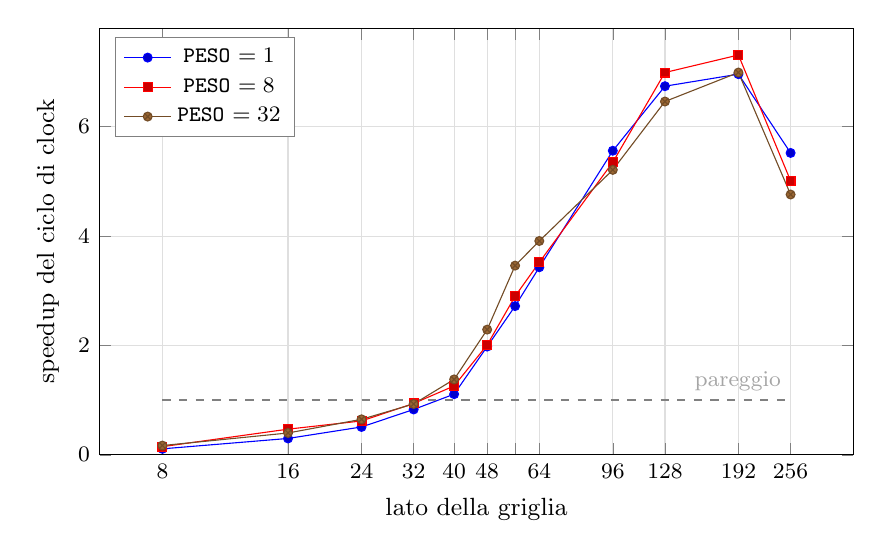
\begin{tikzpicture}
    \begin{axis}[
        width=0.92\textwidth, height=7cm,
        xmode=log, log basis x=2,
        xlabel={lato della griglia}, ylabel={speedup del ciclo di clock},
        xtick={8,16,24,32,40,48,56,64,96,128,192,256},
        xticklabels={8,16,24,32,40,48,,64,96,128,192,256},
        xticklabel style={font=\footnotesize},
        yticklabel style={font=\footnotesize},
        label style={font=\small},
        legend style={font=\footnotesize, at={(0.02,0.98)}, anchor=north west,
                      draw=gray, fill=white},
        ymin=0, ymax=7.8,
        grid=major, grid style={gray!25},
        mark size=1.6pt,
    ]
    % Generato da docs/dati/grafici.py: non modificare a mano.
% Rigenerare con 'make scala' oppure 'make grafici'.

\addplot coordinates {% peso uno
    (8,0.11) (16,0.30) (24,0.51) (32,0.83) (40,1.11) (48,1.98) (56,2.72) (64,3.43) (96,5.56) (128,6.74) (192,6.96) (256,5.52)
};
\addlegendentry{\texttt{PESO} $= 1$}

\addplot coordinates {% peso otto
    (8,0.15) (16,0.47) (24,0.62) (32,0.94) (40,1.26) (48,2.01) (56,2.90) (64,3.52) (96,5.35) (128,6.99) (192,7.31) (256,5.01)
};
\addlegendentry{\texttt{PESO} $= 8$}

\addplot coordinates {% peso trentadue
    (8,0.17) (16,0.40) (24,0.65) (32,0.93) (40,1.38) (48,2.29) (56,3.46) (64,3.91) (96,5.21) (128,6.46) (192,6.99) (256,4.76)
};
\addlegendentry{\texttt{PESO} $= 32$}

    \draw[dashed, thick, gray] (axis cs:8,1) -- (axis cs:256,1);
    \node[font=\footnotesize, anchor=south east, gray!70]
         at (axis cs:256,1) {pareggio};
    \end{axis}
    \end{tikzpicture}
    \caption{Speedup del ciclo di clock contro il lato della griglia: minimo di
             nove ripetizioni, migliore fra le quattro conte di thread parallele
             e rapportato al caso a un thread. Il pareggio letto su questa
             curva è quindi la prima forma in cui \emph{qualche} conta di thread
             supera uno, definizione più permissiva di quella della
             tabella~\ref{tab:crossover}, che è a otto thread fissi. Le tre
             curve corrispondono a tre intensità di calcolo che differiscono di
             un fattore trentadue e attraversano il pareggio fra le stesse due
             forme. Lo scarto residuo fra $40\times40$ e $64\times64$ è il costo
             di creazione dei thread, che a \texttt{ITER} fisso è ammortizzato
             su più cicli dai valori alti di \texttt{PESO}; oltre $96\times96$
             l'ordine delle curve si inverte da una forma all'altra ed è
             dispersione della misura.}
    \label{fig:pareggio}
\end{figure}

Il pareggio, riportato nella figura~\ref{fig:pareggio}, cade a $40\times40$ e non
a $24\times24$, dove la tabella~\ref{tab:crossover} lo colloca. Lo scostamento
ha la stessa origine di quello discusso nella sezione~\ref{sec:parallelo}: la
previsione assume 35\,ns per istruzione, mentre la tabella~\ref{tab:memoria}
ne misura da 16 a 23 nell'intervallo di forme in cui il pareggio cade. Rifatta
con quei valori, la previsione colloca il pareggio appena sotto $40\times40$,
cioè dove è stato misurato: il modello prevede correttamente il punto di
pareggio non appena gli si dà il costo per istruzione della forma giusta.

\pagebreak

La collocazione è stretta e non estrapolata, perché $32\times32$ e
$40\times40$ sono due forme contigue dello sweep e il pareggio cade fra loro per
tutti e tre i valori di \texttt{PESO}: a $32\times32$ le tre curve valgono
$0{,}83\times$, $0{,}94\times$ e $0{,}93\times$, a $40\times40$ $1{,}11\times$,
$1{,}26\times$ e $1{,}38\times$. Sotto il pareggio la perdita è severa, fino a
poco più di un decimo della velocità seriale su $8\times8$: è il regime in cui
cadono tutte le forme della suite di verifica, e spiega le misure della
sezione~\ref{sec:parallelo}.

Il confronto fra le tre curve dà un risultato negativo. Il pareggio cade
fra le stesse due forme per tutti e tre i valori di \texttt{PESO}, che è la
grandezza in questione, e il valore $\texttt{PESO}=32$ esegue trentadue volte le
istruzioni di calcolo per comunicazione di $\texttt{PESO}=1$ senza spostarlo di
una forma. Le tre curve restano ordinate per \texttt{PESO} sulla maggior parte
delle forme, con uno scarto che fra $40\times40$ e $64\times64$ arriva al
25\,\%, ma quell'ordinamento non è intensità di calcolo: è il costo di creazione
dei thread, che a \texttt{ITER} fisso i valori alti di \texttt{PESO} ammortizzano
su più cicli, perché eseguono più cicli. Il controllo riportato più sotto rimuove
proprio questa differenza e non lascia un effetto residuo che la misura risolva. Se ne conclude che
l'efficienza della parallelizzazione non dipende da che cosa l'array calcola,
ma solo da quanto è grande.

La ragione è strutturale e discende dal disegno del ciclo di clock. Un ciclo è
per costruzione \emph{una istruzione per cella}: qualunque cosa le celle stiano
eseguendo, \texttt{grid\_step} apre due regioni parallele, esegue $R \cdot C$
istruzioni e aggiorna $4 R \cdot C$ canali. Il lavoro per ciclo, e quindi il suo
rapporto con il costo delle due barriere, dipende soltanto da $R \cdot C$. Un
programma a maggiore intensità di calcolo non rende più pesante il ciclo, ne
esegue semplicemente di più, e il numero di cicli si semplifica nel rapporto fra
tempo seriale e tempo parallelo.

Il controllo diretto separa le due cose, ed è uno sweep a sé. Confrontando
\texttt{PESO} $=1$ con \texttt{ITER} $=62$ e \texttt{PESO} $=32$ con
\texttt{ITER} $=8$, che eseguono 2624 cicli entrambi pur differendo di
trentadue volte nelle istruzioni di calcolo per comunicazione, lo speedup a otto
thread è $0{,}78\times$ contro $0{,}77\times$ su $32\times32$ e $1{,}91\times$
contro $2{,}20\times$ su $48\times48$. Su $32\times32$ i due coincidono; su
$48\times48$ i minimi distano il 15\,\%, ma le cinque ripetizioni delle due
condizioni si sovrappongono, quindi la misura non risolve la differenza. A
parità di cicli l'intensità di calcolo non produce un effetto misurabile. Il
vantaggio che i valori alti di \texttt{PESO} mostrano nella
figura~\ref{fig:pareggio}, dove è fisso \texttt{ITER} e non il numero di cicli,
è il costo di creazione dei thread ammortizzato su più cicli.

È una proprietà del simulatore e non dell'array simulato, e ha una conseguenza
operativa: per spostare il pareggio non serve un programma diverso, serve una
griglia più grande oppure una regione parallela che non si riapra a ogni ciclo,
che è la seconda delle due modifiche indicate nelle conclusioni.

La frazione seriale conferma l'altra faccia dello stesso conto: passa dal
$10{,}1\,\%$ su $8\times8$ allo $0{,}64\,\%$ su $256\times256$, coerente con un
ingresso/uscita di perimetro che cresce come $O(R+C)$ contro un lavoro utile che
cresce come $O(R \cdot C)$. Il tetto di Amdahl si allontana esattamente nella
direzione in cui l'array diventa conveniente.

\pagebreak

I limiti della misura sono severi, e discendono dalle caratteristiche della
macchina riportate nella tabella~\ref{tab:macchina}: l'asimmetria fra core
prestazionali e core efficienti, il regolatore di frequenza in modalità di
risparmio e il fatto che la macchina non sia dedicata rendono il valore
assoluto dello speedup non riproducibile fra sessioni diverse. Lo sweep
ripetuto a distanza di ore e di giorni ha infatti dato picchi di
$3{,}7\times$, $7{,}3\times$ e
$8{,}5\times$. Si sono invece ritrovate in ogni sessione la collocazione del
pareggio, la severità della perdita sotto di esso, l'andamento della frazione
seriale e l'indipendenza da \texttt{PESO}. Del grafico è quindi significativa la
forma della curva, non il valore puntuale di ciascun punto.

\subsection{Il muro della memoria}
\label{sec:memoria}

Il pareggio è raggiungibile: $40\times40$ occupa 27\,MB e
$256\times256$ poco più di un gigabyte. Quello che resta fuori portata è il
regime asintotico. La struttura di una cella occupa 16\,632 byte, di cui
16\,384 sono la memoria privata: una griglia $1000 \times 1000$ richiederebbe
15,5\,GiB ed è quindi irraggiungibile allo stato attuale.

Il costo però non è solo di capacità, ed è misurabile separatamente. Il passo di
16\,KB fra celle contigue fa sì che lo stato caldo di ogni cella, poche decine
di byte fra registri e canali, cada su una pagina diversa: su $256\times256$
sono 65\,536 pagine contro un \emph{buffer} di traduzione che ne indirizza
qualche migliaio. L'effetto si isola facendo crescere la griglia a un solo
thread, dove OpenMP non entra affatto in gioco e nessuna delle cause discusse
finora può intervenire, e la tabella~\ref{tab:memoria} lo riporta.

\begin{table}[htbp]
    \centering
    \begin{tabular}{lrr}
        \toprule
        griglia & memoria occupata & costo per cella-ciclo \\
        \midrule
        $16\times16$   & 4\,MB     & 17,1\,ns \\
        $32\times32$   & 17\,MB    & 15,9\,ns \\
        $48\times48$   & 38\,MB    & 22,8\,ns \\
        $64\times64$   & 68\,MB    & 28,5\,ns \\
        $96\times96$   & 153\,MB   & 28,9\,ns \\
        $128\times128$ & 272\,MB   & 33,1\,ns \\
        $192\times192$ & 613\,MB   & 63,5\,ns \\
        $256\times256$ & 1090\,MB  & 83,4\,ns \\
        \bottomrule
    \end{tabular}
    \caption{Degrado da sola località, minimo di tre ripetizioni a un thread. Il
             numero di iterazioni è scalato per forma in modo che ogni misura
             duri fra uno e due secondi fino a $128\times128$ e fino a quattro
             sulle due forme maggiori, così che le righe siano confrontabili fra
             loro: lo scarto fra ripetizioni resta sotto il 9\,\%.}
    \label{tab:memoria}
\end{table}

Il costo di simulare una istruzione passa da 15,9 a 83,4\,ns, cioè più che
quintuplica, senza che sia cambiato nulla nel lavoro da fare:
le stesse istruzioni, lo stesso programma, un solo thread. Il salto netto è fra
$32\times32$ e $48\times48$, dove il costo cresce del 43\,\%: sono l'ultima
forma che entra ancora nella cache di ultimo livello, che su questa macchina è
di 24\,MB (tabella~\ref{tab:macchina}), e la prima che non ci entra. Il minimo
fra $16\times16$ e $32\times32$ è invece di appena il 7,5\,\%, cioè dentro la
dispersione dichiarata nella didascalia, e la misura non lo risolve. Come ogni
misura di tempo, il
fattore dipende dalla sessione, e in sessioni diverse è stato di tre e di cinque
volte; quello che si ritrova in ogni sessione è il salto in corrispondenza della
capacità della cache e la crescita monotona oltre di esso.

Ridurre la memoria privata non è però il rimedio, e la misura diretta lo mostra:
ricompilando con 1\,KB per cella invece di 16\,KB, cioè riducendo di sedici
volte l'occupazione, su $128\times128$ il tempo a un thread migliora solo del
$5\,\%$. Il numero di pagine su cui cade lo stato caldo scende, perché con
celle da 1\,KB quattro celle condividono una pagina da 4\,KB, ma scende solo di
quattro volte, da circa sedicimila a circa quattromila su $128\times128$, e
resta di un ordine di grandezza sopra il buffer di traduzione. Il regime non
cambia, ed è per questo che il guadagno è del cinque per cento e non
proporzionale alla riduzione. Rendere parametrica la memoria privata sblocca
quindi le griglie grandi, ma non rende più veloci quelle che già ci stanno.

\clearpage
\subsection{Correttezza}

L'aggiornamento a due fasi rende il
risultato parallelo bit-identico a quello seriale, quindi la verifica è la
stessa: rigenerare tutti i dati al variare del numero di thread e pretendere che
il confronto resti vuoto. Una differenza in uno dei file non sarebbe un problema
di prestazioni ma una violazione del determinismo.

Lo sweep dei tempi la esercita per intero senza che serva un controllo a parte,
perché esegue i sei programmi con uno, due, quattro, otto e sedici thread
mantenendo attive le asserzioni dei programmi di verifica: quattrocento
esecuzioni, tutte superate. Le colonne di conteggio non si muovono di una cifra
fra una conta di thread e l'altra, e non si sono mosse nemmeno fra sessioni di
misura che pure hanno dato tempi diversi: i conteggi sono riproducibili
esattamente, i tempi solo come forma della curva.

\ifconclusioni% !TEX root = Tesi_Corsi_Leonardo_656276.tex
\chapter{Conclusioni e sviluppi futuri}
\label{ch:conclusioni}

Il lavoro consegna due risultati, uno sull'array simulato e uno sul simulatore
che lo esegue. Il primo riguarda il canale ed è il principio enunciato nel
capitolo~\ref{ch:introduzione}; il secondo riguarda il ciclo di clock
parallelizzato e ne individua il regime di convenienza. Le due sezioni che
seguono li riprendono uno per uno, la terza indica gli sviluppi che le misure
lasciano aperti.

\section{Il \emph{ready bit} al posto della schedulazione}
\label{sec:sintesi-finale}

Il principio enunciato nel capitolo~\ref{ch:introduzione} è verificato nella
forma seguente. Sullo stesso programma e con gli stessi parametri, il risultato
ottenuto con il \emph{ready bit} è corretto per ogni velocità relativa dei nodi e
per ogni lunghezza della catena; senza, è corretto soltanto quando il consumatore
è abbastanza veloce, e negli altri casi l'array produce un risultato
numericamente definito ma errato, che nessun componente rileva. Ciascun lato del
canale commuta soltanto il proprio registro da un bit ed è il confronto fra i
due, e non il valore dell'uno o dell'altro, a stabilire se il canale sia pieno o
vuoto: nessuno dei due lati conosce il comportamento temporale dell'altro, e la
correttezza cessa di dipendere dalla schedulazione con cui l'host alimenta
l'array.

Il costo si misura su due assi. In cicli è nullo: da ritardo uno in poi le due
modalità impiegano lo stesso numero di cicli, perché il tempo lo
consuma il consumatore lento e non il protocollo; a ritardo zero il
\emph{lockstep} risparmia otto cicli su quarantacinque, ed è anche l'unica
configurazione in cui non perde dati, cioè l'unica in cui il \emph{ready bit}
non serviva. In area lo quantifica la sintesi del
modello RTL (sezione~\ref{sec:rtl}): 66 flip-flop e 6 porte
combinatorie per canale, di cui 64 flip-flop sono i due registri dati da 32 bit
e due sono i contatori, mentre le sei porte sono lo XOR e lo XNOR dei due
comparatori più quattro abilitazioni. Lo stato di sincronizzazione in senso
stretto è quindi di due flip-flop per canale, mentre il secondo registro dati è
una conseguenza dell'asimmetria fra \texttt{OUT} e \texttt{SETRDY}, poiché il
valore appena caricato e quello pubblicato e non ancora letto possono differire
nello stesso istante. Fra due celle adiacenti corrono 68 fili.

\section{L'efficienza della parallelizzazione dipende dalla sola dimensione
         della griglia}

Il secondo risultato riguarda il simulatore. Il ciclo di clock si parallelizza
senza una sola sezione critica, e il guadagno che se ne ottiene è determinato
dal solo prodotto $R \cdot C$: il lavoro di un ciclo sono $R \cdot C$ istruzioni
simulate, il costo da pagare per distribuirlo sono le due regioni parallele che
il ciclo apre, e il pareggio cade dove le due grandezze si eguagliano.

Il pareggio è misurato a $40\times40$, e la sezione~\ref{sec:pareggio} mostra
che la collocazione è stretta perché cade fra due forme contigue dello sweep
per tutti e tre i valori dell'intensità di calcolo. La previsione analitica lo
collocava a $24\times24$, ma lo scostamento non è del modello: la previsione
assume un costo per istruzione simulata misurato su una griglia molto più
grande, dove la località è peggiore, e rifatta con il costo della forma giusta
colloca il pareggio dove è stato misurato. Il modello analitico e la misura
concordano quindi sia sul rapporto a $12\times12$ sia sul punto di pareggio.

Che l'intensità di calcolo non compaia in quel rapporto discende dal disegno del
ciclo di clock, che è per costruzione \emph{una istruzione per cella}: il numero
di cicli si semplifica nel rapporto fra tempo seriale e tempo parallelo. Il
programma \texttt{pesante}
(sezione~\ref{sec:kernel-pesante}) verifica questa proprietà dove sarebbe più
visibile smentirla: trentadue volte le istruzioni di calcolo per ogni
comunicazione non spostano il pareggio di una forma, e il controllo a parità di
cicli non lascia un effetto residuo che la misura risolva. La misura del
pareggio si estende quindi ai programmi in cui le celle terminano insieme: per
questi, al di sopra di $40\times40$ l'aggiunta di thread accelera il ciclo di
clock qualunque cosa stiano eseguendo, e non occorre rimisurare il pareggio per
ognuno. Resta fuori il caso della terminazione sfalsata, perché la fase di
calcolo salta le celle già ferme e il lavoro per ciclo scende allora sotto
$R \cdot C$ distribuendosi male su una ripartizione statica; entrambi i
programmi su cui il pareggio è misurato hanno terminazione uniforme, quindi la
suite non lo esercita. La conseguenza
operativa è che per spostarlo non serve un programma diverso, serve una griglia
più grande oppure una regione parallela che non si riapra a ogni ciclo.

Le forme della suite di verifica si fermano a $12\times12$ e cadono quindi tutte
al di sotto del pareggio, dove la perdita arriva a poco più di un decimo della
velocità seriale. Sono le dimensioni che il compito di quello sweep richiede,
per la ragione data nella sezione~\ref{sec:metodologia}: quello sweep verifica
la correttezza e non le prestazioni.

Il tetto asintotico non è quello di Amdahl ma la località. La frazione
seriale scende dal $10{,}1\,\%$ su $8\times8$ allo $0{,}64\,\%$ su
$256\times256$, cioè si allontana esattamente nella direzione in cui l'array
diventa conveniente; nella stessa direzione il costo di simulare una istruzione
più che quintuplica, da 15,9 a 83,4\,ns, a un solo thread e a parità di lavoro
da svolgere, perché il passo di 16\,KB fra celle contigue disperde lo stato caldo
di ciascuna su una pagina diversa.

Il limite di queste misure è quello posto nella sezione~\ref{sec:pareggio}: la
macchina non è dedicata e il valore assoluto dello \emph{speedup} non è
riproducibile fra sessioni diverse. Si ritrovano invece in ogni sessione la
collocazione del pareggio, la severità della perdita al di sotto di esso,
l'andamento della frazione seriale e l'indipendenza dall'intensità di calcolo,
che sono le quattro affermazioni su cui il risultato poggia.

\section{Sviluppi futuri}
\label{sec:sviluppi}

Gli sviluppi possibili si dispongono su due piani. Le prime due modifiche non
sono scelte di progetto ma conseguenze dirette delle misure del
capitolo~\ref{ch:risultati}, e restano dentro il modello attuale. Le altre tre
lo estendono e ne mettono in discussione altrettante ipotesi, cioè la
profondità unitaria dei canali, il clock unico e il confine oltre il quale il
modello RTL si ferma.

\subsection{Le due modifiche indicate dalla misura}

Le prime due estensioni non sono scelte di progetto ma indicazioni che i dati
del capitolo~\ref{ch:risultati} lasciano aperte. Spostare il contatore di
lettura nella cella consumatrice ridurrebbe il \emph{false sharing} e
allineerebbe al tempo stesso il codice C alla struttura fisica del circuito,
dove quel flip-flop starebbe nel consumatore: due criteri indipendenti indicano
la stessa modifica, e non costa area, perché il contatore passa da un modulo
all'altro senza cambiare di numero. Non lo eliminerebbe, per la ragione data
nella sezione~\ref{sec:parallelo}, e richiede di decidere a chi spetti
l'aggiornamento di fine ciclo di quel campo, che oggi è del proprietario del
canale. Spostare la regione parallela fuori dal ciclo dei passi pagherebbe due
barriere invece di due per ciclo, ed è il modo di abbassare il pareggio senza
ingrandire la griglia.

\subsection{Canali di profondità maggiore di uno}

Portare la profondità da uno a $N$ è una estensione ortogonale: i due contatori
diventerebbero modulo $N$ invece che modulo due e il resto del protocollo non
cambierebbe di una riga. La misura da fare è quanta parte della differenza fra
le due modalità sopravvive quando il buffer nasconde il disallineamento.

\subsection{Clock indipendenti}

Il modello è sincrono, con un clock globale. Un modello asincrono vero
richiederebbe di cambiare il solo ciclo di simulazione e non il protocollo,
perché il \emph{ready bit} compensa il disallineamento del carico di lavoro e
non quello del clock.

\subsection{Il resto della cella in RTL}

Oggi il modello hardware copre il canale e l'interfaccia di comunicazione.
Estenderlo al processore completerebbe il confronto e permetterebbe di misurare
l'area dell'intera cella e non della sola interfaccia.
\fi

\bibliographystyle{plain} % We choose the "plain" reference style
\bibliography{bibliography} % Entries are in the refs.bib file
%\addbibresource{bibliography.bib}
%\printbibliography

\end{document}
